\documentclass[10pt,a4paper]{article}
\usepackage[utf8]{inputenc}
\usepackage{graphicx}
\def\Pr{\mathop{\rm Pr}}
\usepackage[landscape,margin=1cm]{geometry}
\usepackage[english]{babel}
\usepackage{tikz}
\usetikzlibrary{arrows,snakes,backgrounds,shapes.geometric}
\title{Neuromatch Academy Pre-Requisite Refresher - Summary Sheet}
\author{Neuromatch}
%\date{July 2019}
\usepackage[default]{raleway}
\usepackage{fontawesome}
\usepackage[T1]{fontenc}

\usepackage{hyperref}
\usepackage{enumitem}
\usepackage{lipsum}

\usepackage{xcolor}
\definecolor{customcolor}{HTML}{616AC5}
\definecolor{alert}{HTML}{CD5C5C}
\definecolor{w3schools}{HTML}{4CAF50}
\definecolor{subbox}{gray}{0.60}
\definecolor{codecolor}{HTML}{FFC300}
\colorlet{xx}{customcolor}


%--------------------------Editor mode.

\usepackage
[citestyle=authoryear,
sorting=nty,	  		%Sorts bibliography by year, name, title
autocite=footnote, 		%Autocite command generates footnotes
autolang=hyphen, 		
mincrossrefs=1, 	
backend=biber]
{biblatex}

\DeclareFieldFormat{postnote}{#1}
\DeclareFieldFormat{multipostnote}{#1}
\DeclareAutoCiteCommand{footnote}[f]{\footcite}{\footcites}

\bibliography{literature}
%----------------------------------------
%--------------------------------------------------------------------------------
\usepackage{tcolorbox}

\tcbuselibrary{most,listingsutf8,minted}

\tcbset{tcbox width=auto,left=1mm,top=1mm,bottom=1mm,
right=1mm,boxsep=1mm,middle=1pt}

\newenvironment{mycolorbox}[2]{%
\begin{tcolorbox}[grow to left by=-1em,grow to right by=-1em,capture=minipage,fonttitle=\large\bfseries, enhanced jigsaw,boxsep=1mm,colback=#1!30!white,on line,tcbox width=auto, toptitle=0mm,colframe=#2,opacityback=0.7,nobeforeafter,title=#2]%
}{\end{tcolorbox}\\[0.2em]}

\newenvironment{subbox}[2]{%
\begin{tcolorbox}[capture=minipage,fonttitle=\normalsize\bfseries, enhanced jigsaw,boxsep=1mm,colback=#1!30!white,on line,tcbox width=auto,left=0.3em,top=1mm, toptitle=0mm,colframe=#1,opacityback=0.7,nobeforeafter,title=#2]\footnotesize %
}{\normalsize\end{tcolorbox}\vspace{0.1em}}

\newenvironment{multibox}[1]{%
\begin{tcbraster}[raster columns=#1,raster equal height,nobeforeafter,raster column skip=1em,raster left skip=1em,raster right skip=1em]}{\end{tcbraster}}

\newenvironment{textbox}[1]{\begin{mycolorbox}{customcolor}{#1}}{\end{mycolorbox}}

%-------------------------------
\newtcblisting{codebox}[2]{colback=codecolor!5,colframe=codecolor!80!black,listing only, 
minted options={numbers=left,style=tcblatex,fontsize=\normalsize,breaklines,autogobble,linenos,numbersep=1mm},
left=5mm,enhanced,
title=#2, fonttitle=\bfseries,
listing engine=minted,minted language=#1}

%--------------------------------------------------------------------------------
\newcommand{\punkti}{~\lbrack\dots\rbrack~}

\renewenvironment{quote}
               {\list{\faQuoteLeft\phantom{ }}{\rightmargin\leftmargin}%
                \item\relax\scriptsize\ignorespaces}
               {\unskip\unskip\phantom{xx}\faQuoteRight\endlist}
               

%--------------------------------------------------------------------------------
\newcommand{\bgupper}[3]{\colorbox{#1}{\color{#2}\huge\bfseries\MakeUppercase{#3}}}
\newcommand{\bg}[3]{\colorbox{#1}{\bfseries\color{#2}#3}}

\newcommand{\mycommand}[2]{{\ttfamily\detokenize{#1}}~\dotfill{}~{\footnotesize #2}\\}
\newcommand{\sep}{{\scriptsize~\faCircle{ }~}}


\newcommand{\bggreen}[1]{\medskip\bgupper{w3schools}{black}{#1}\\[0.5em]}
\newcommand{\green}[1]{\smallskip\bg{w3schools}{white}{#1}\\}
\newcommand{\red}[1]{\smallskip\bg{alert}{white}{#1}\\}

\usepackage{multicol}
\setlength{\columnsep}{30pt}

\setlength{\parindent}{0pt}
\pagestyle{empty}

\usepackage{csquotes}

\newcommand{\loremipsum}{Lorem ipsum dolor sit amet.}

\clearpage

%--------------------------------------------------------------------------------
\begin{document}


%\section{Data Type}
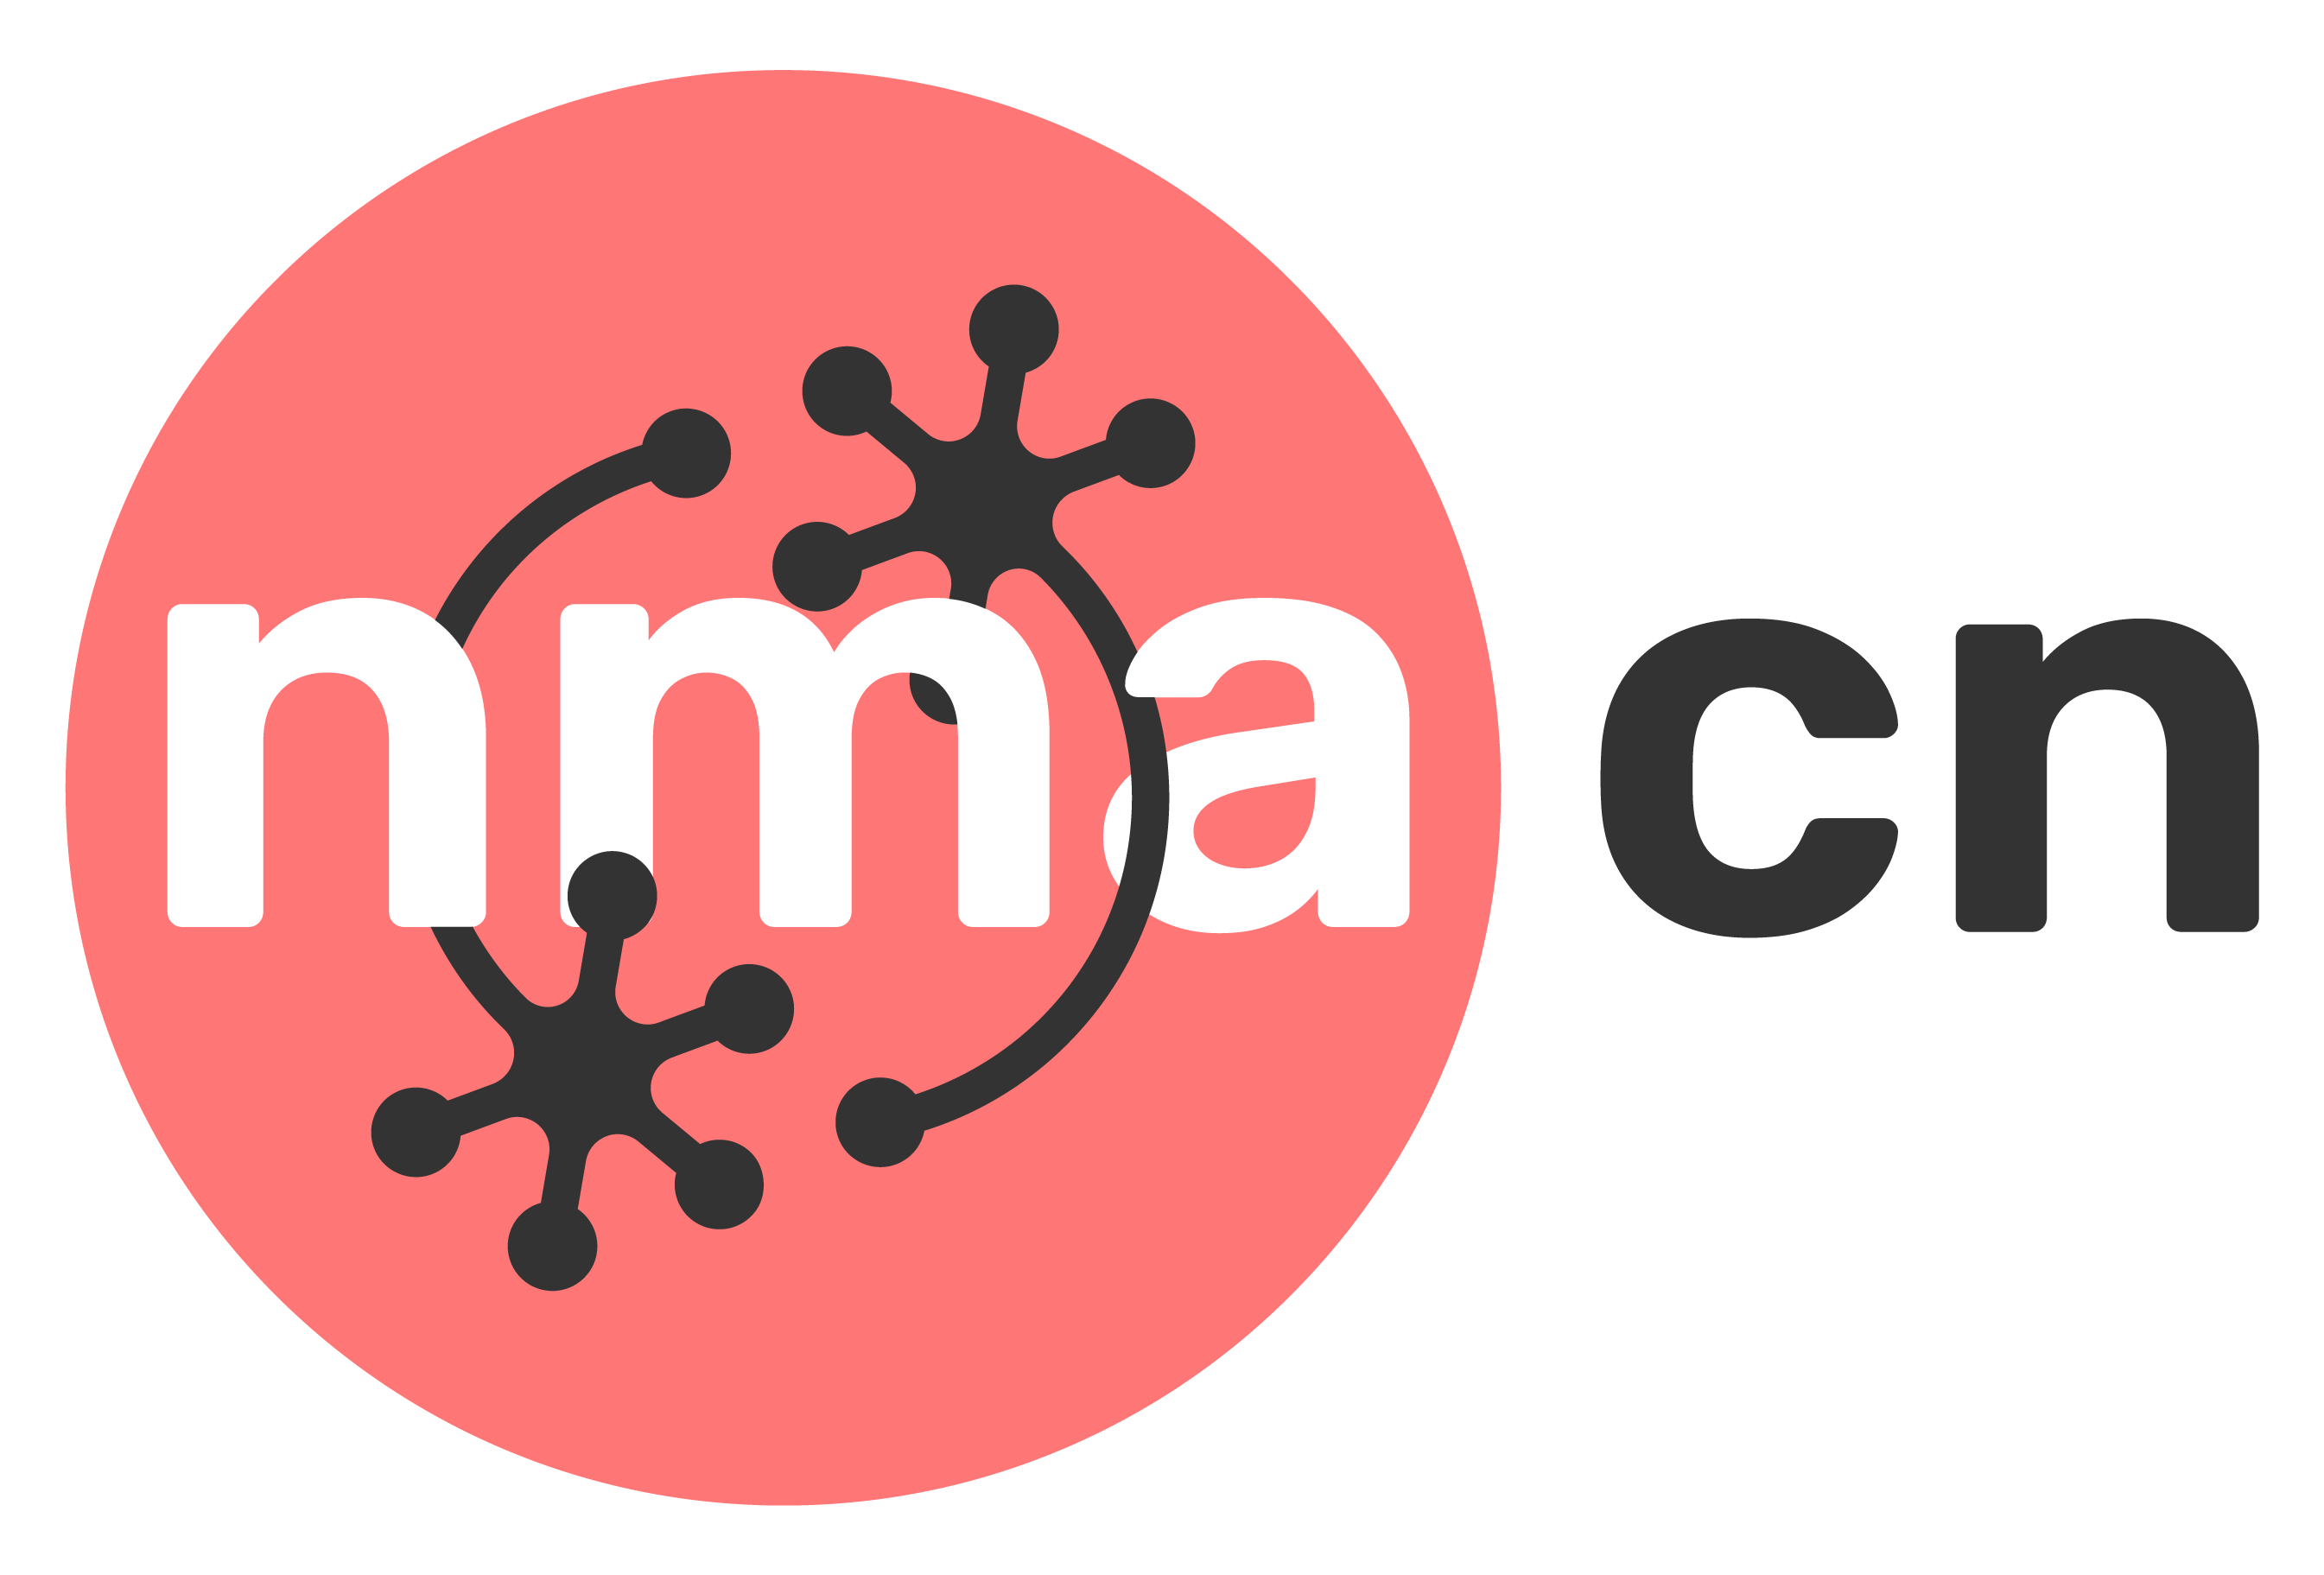
\includegraphics[scale=0.03]{Figures/NMACN.png}\href{https://compneuro.neuromatch.io/tutorials/intro.html}{\textbf{\Huge{Neuromatch Academy: Model Fitting - Summary Sheet}}\footnote{’t Hart et al., (2022). Neuromatch Academy: a 3-week, online summer school in computational neuroscience. Journal of Open Source Education, 5(49), 118. https://doi.org/10.21105/jose.00118}}
%$\subsection*{Cheat Sheet}
\small
\begin{multicols}{3}
%\scriptsize
%\pagecolor{black}
\let\clearpage\relax
\begin{textbox}{\href{https://compneuro.neuromatch.io/tutorials/W1D2_ModelFitting/student/W1D2_Intro.html}{Linear regression with MSE }}
\begin{subbox}{subbox}{Mean Squared Error (MSE)}
\scriptsize
\textbf{Linear least squares regression} is an old but gold  optimization procedure that we are going to use for data fitting. Least squares (LS) optimization problems are those in which the objective function is a quadratic function of the
parameter(s) being optimized.

Suppose you have a set of measurements: for each data point or measurement, you have $y_{i}$ (the "dependent" variable) obtained for a different input value, $x_{i}$ (the "independent" variable).  Suppose we believe the measurements are proportional to the input values, but are corrupted by some (random) measurement errors, $\epsilon_{i}$, that is:
\begin{equation}
y_{i}= \theta x_{i}+\epsilon_{i}
\end{equation}
for some unknown slope parameter $\theta.$ The least squares regression problem uses \textbf{mean squared error (MSE)} as its objective function, it aims to find the value of the parameter $\theta$ by minimizing the average of squared errors:
\begin{equation}
\min _{\theta} \frac{1}{N}\sum_{i=1}^{N}\left(\epsilon_{i}\right)^{2}
\end{equation}
\begin{equation}
\min _{\theta} \frac{1}{N}\sum_{i=1}^{N}\left(y_{i}-\theta x_{i}\right)^{2}
\end{equation}
\centering
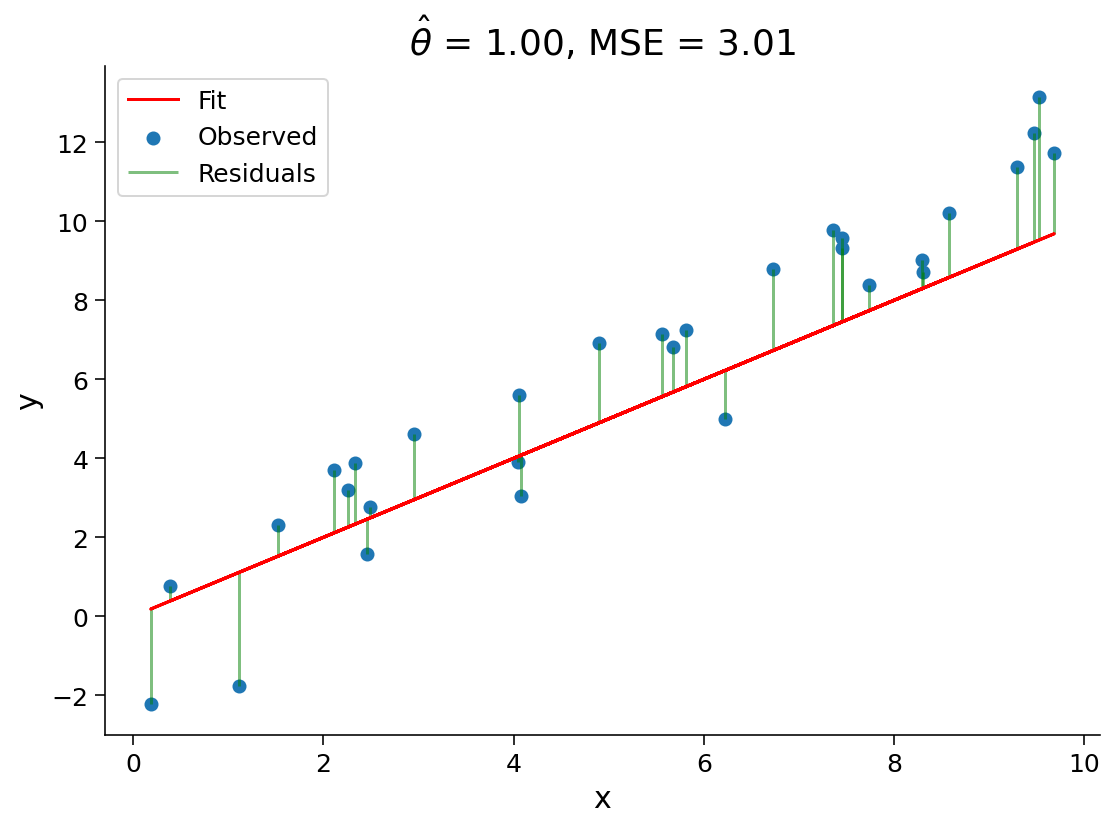
\includegraphics[scale=0.15]{Figures/ModelFitting/MFFigure1.png}
\end{subbox}
%%%%%%%%%%%%%%%%%%%%%%%%%%%%%%%%%%%%%%%%%%%%%%%%%%
\begin{subbox}{subbox}{Least-Squares Optimization}
\scriptsize
The MSE value relies on a grid of hand-specified values. If we didn't pick a good range to begin with, or with enough granularity, we might miss the best possible estimator. Instead of finding the minimum MSE from a set of candidate estimates, let's solve for it analytically.
We can do this by minimizing the cost function. Mean squared error is a convex objective function, therefore we can compute its minimum using calculus for find the best estimate: \begin{align}
\hat\theta = \frac{\mathbf{x}^\top \mathbf{y}}{\mathbf{x}^\top \mathbf{x}}
\end{align}

where $\mathbf{x}$ and $\mathbf{y}$ are vectors of data points.

\end{subbox}

\end{textbox}
%%%%%%%%%%%%%%%%%%%%%%%%% 
%%%%%%%%%%%%%%%%%%%%%%%%%
\begin{textbox}{\href{https://compneuro.neuromatch.io/tutorials/W1D2_ModelFitting/student/W1D2_Intro.html}{Linear regression with MLE }  }
\begin{subbox}{subbox}{ Gaussian noise}
\scriptsize
In the MSE we made the assumption that the data was drawn from a linear relationship with noise added.

In that case we treated the noise as simply a nuisance, but what if we factored it directly into our model?

The noise component $\epsilon$ is often modeled as a random variable drawn from a Gaussian distribution (also called the normal distribution).

The Gaussian distribution is described by its probability density function (pdf)
\begin{align}
\mathcal{N}(x; \mu, \sigma^2) = \frac{1}{\sqrt{2\pi\sigma^2}}e^{-\frac{1}{2\sigma^2}(x-\mu)^2}
\end{align}

and is dependent on two parameters: the mean $\mu$ and the variance $\sigma^2$. We often consider the noise signal to be Gaussian "white noise", with zero mean and unit variance
$\epsilon \sim \mathcal{N}(0, 1).
$

\end{subbox}
%%%%%%%%%%%%%%%%%%%%%%%%%%%%%%%%%%%%%%%%%%%%%%%%%%
\begin{subbox}{subbox}{Probabilistic Models}
\scriptsize
Consider again our simplified model $y = \theta x + \epsilon$ where the noise has zero mean and unit variance $\epsilon \sim \mathcal{N}(0, 1)$. We can now also treat $y$ as a random variable drawn from a Gaussian distribution where $\mu = \theta x$ and $\sigma^2 = 1$, 
$y \sim \mathcal{N}(\theta x, 1),
$

which is to say that the probability of observing $y$ given $x$ and parameter $\theta$ is
\begin{align}
p(y|x,\theta) = \frac{1}{\sqrt{2\pi}}e^{-\frac{1}{2}(y-\theta x)^2}
\end{align}

\end{subbox}

\begin{subbox}{subbox}{Likelihood Estimation}
\scriptsize
 Given the inherent uncertainty when dealing in probabilities, we talk about the likelihood that some estimate $\hat{\theta}$ fits our data. The likelihood function $\mathcal{L}(\theta)$ is equal to the probability density function parameterized by that $\theta$:
\begin{align}
\mathcal{L}(\theta|x,y) = p(y|x,\theta) = \frac{1}{\sqrt{2\pi\sigma^2}}e^{-\frac{1}{2\sigma^2}(y-\theta x)^2}
\end{align}
Since we have assumed that the noise affects each output independently, we can factorize the likelihood, and write:
\begin{align}
\mathcal{L}(\theta|\mathbf{x}, \mathbf{y}) = \prod_{i=1}^N \mathcal{L}(\theta|x_i,y_i),
\end{align}
where we have $N$ data points $\mathbf{x} = [x_1,...,x_N]$ and $\mathbf{y} = [y_1,...,y_N]$.
\end{subbox}
\end{textbox}
%%%%%%%%%%%%%%%%%%%%%%%%% 
%%%%%%%%%%%%%%%%%%%%%%%%%
\begin{textbox}{\href{https://compneuro.neuromatch.io/tutorials/W1D2_ModelFitting/student/W1D2_Intro.html}{Linear regression with MLE }   }
\begin{subbox}{subbox}{Finding the Maximum Likelihood Estimator (MLE)}
\scriptsize
We want to find the parameter value $\hat\theta$ that makes our data set most likely:

\begin{align}
\hat{\theta}_{\textrm{MLE}} = \underset{\theta}{\operatorname{argmax}} \mathcal{L}(\theta|X,Y) 
\end{align}

We discussed how taking the logarithm of the likelihood helps with numerical stability, the good thing is that it does so without changing the parameter value that maximizes the likelihood. Indeed, the $\log()$ function is *monotonically increasing*, which means that it preserves the order of its inputs. So we have:

\begin{align}
\hat{\theta}_{\textrm{MLE}} = \underset{\theta}{\operatorname{argmax}} \sum_{i=1}^m \textrm{log} \mathcal{L}(\theta|x_i,y_i) 
\end{align}

Now substituting our specific likelihood function and taking its logarithm, we get:
\begin{align}
\hat{\theta}_{\textrm{MLE}} = \underset{\theta}{\operatorname{argmax}} [-\frac{N}{2} \operatorname{log} 2\pi\sigma^2 - \frac{1}{2\sigma^2}\sum_{i=1}^N (y_i-\theta x_i)^2].
\end{align}

Note that maximizing the log likelihood is the same as minimizing the negative log likelihood (in practice optimization routines are developed to solve minimization not maximization problems). Because of the convexity of this objective function, we can take the derivative of our negative log likelihhood, set it to 0, and solve - just like our solution to minimizing MSE.

\begin{align}
\frac{\partial\operatorname{log}\mathcal{L}(\theta|x,y)}{\partial\theta}=\frac{1}{\sigma^2}\sum_{i=1}^N(y_i-\theta x_i)x_i = 0
\end{align}
\centering
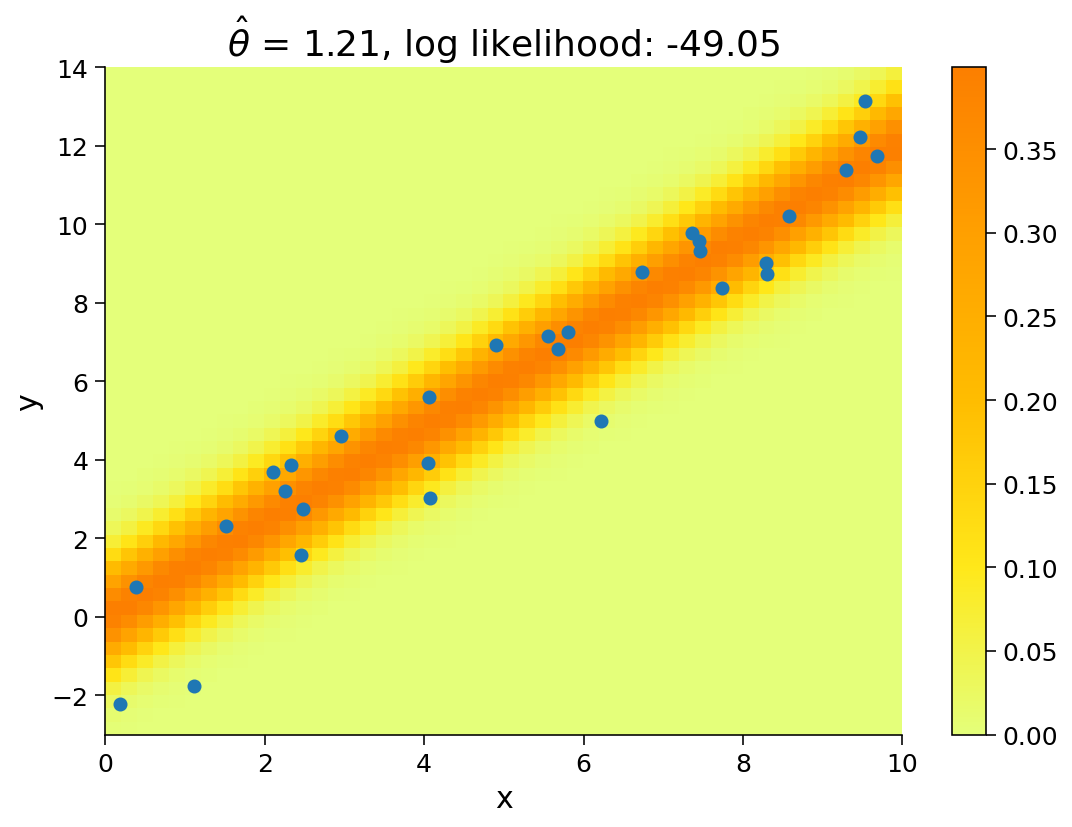
\includegraphics[scale=0.2]{Figures/ModelFitting/MFFigure2.png}
\end{subbox}
\end{textbox}
%%%%%%%%%%%%%%%%%%%%%%%%% 
%%%%%%%%%%%%%%%%%%%%%%%%%
\begin{textbox}{\href{https://compneuro.neuromatch.io/tutorials/W1D2_ModelFitting/student/W1D2_Intro.html}{ Confidence Intervals and Bootstrapping and Cross-validation}}
\begin{subbox}{subbox}{\href{https://compneuro.neuromatch.io/tutorials/W1D3_ModelFitting/student/W1D3_Tutorial3.html}{Confidence Intervals and Bootstrapping }  }

\scriptsize

 Bootstrapping is a resampling procedure that allows to build confidence intervals around inferred parameter values.
It is a widely applicable and very practical method that relies on computational power and pseudo-random number generators (as opposed to more classical approaches than depend on analytical derivations)

The idea is to generate many new synthetic datasets from the initial true dataset by randomly sampling from it, then finding estimators for each one of these new datasets, and finally looking at the distribution of all these estimators to quantify our confidence.

Note that each new resampled datasets will be the same size as our original one, with the new data points sampled with replacement i.e. we can repeat the same data point multiple times. 

\centering
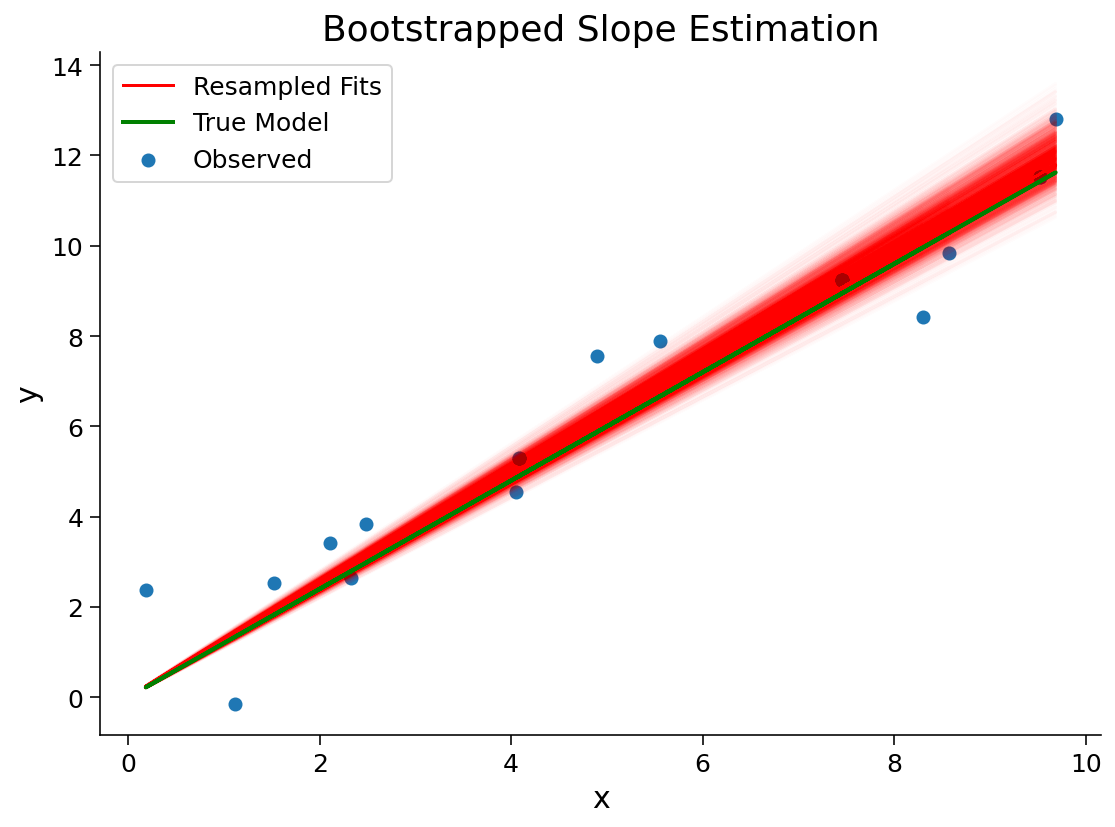
\includegraphics[scale=0.2]{Figures/ModelFitting/MFFigure3.png}

\end{subbox}
\begin{subbox}{subbox}{\href{https://compneuro.neuromatch.io/tutorials/W1D2_ModelFitting/student/W1D2_Tutorial6.html}{Cross-validation (W1D3T6)}  }

\scriptsize

A commonly used method for model selection is to ask how well the model predicts new data that it hasn't seen yet. But we don't want to use test data to do this, otherwise that would mean using it during the training process! One approach is to use another kind of held-out data which we call \textbf{validation data}: we do not fit the model with this data but we use it to select our best model.

We often have a limited amount of data though (especially in neuroscience), so we do not want to further reduce our potential training data by reassigning some as validation. Luckily, we can use \textbf{k-fold cross-validation}! In k-fold cross validation, we divide up the training data into k subsets (that are called \textit{folds}, see diagram below), train our model on the first k-1 folds, and then compute error on the last held-out fold.

\centering
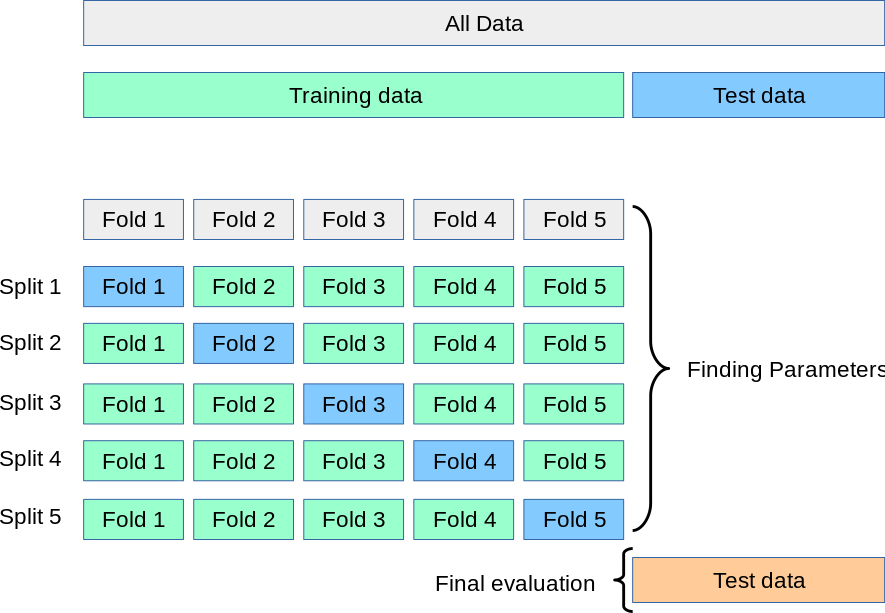
\includegraphics[scale=0.14]{Figures/ModelFitting/MFFigure7.png}

\end{subbox}
\end{textbox}
%%%%%%%%%%%%%%%%%%%%%%%%% 
%%%%%%%%%%%%%%%%%%%%%%%%%
%%%%%%%%%%%%%%%%%%%%%%%%% 
%%%%%%%%%%%%%%%%%%%%%%%%%
\begin{textbox}{\href{https://compneuro.neuromatch.io/tutorials/W1D2_ModelFitting/student/W1D2_Tutorial4.html}{Multiple Linear Regression and Polynomial Regression }   }
\begin{subbox}{subbox}{Multiple Linear Regression}
\scriptsize

We can easily extend univariate regression to the multivariate scenario by adding another parameter for each additional feature
\begin{align}
y = \theta_0 + \theta_1 x_1 + \theta_2 x_2 + ... +\theta_d x_d + \epsilon
\end{align}
where $\theta_0$ is the intercept and $d$ is the number of features (it is also the dimensionality of our input).

We can condense this succinctly using vector notation for a single data point
\begin{align}
y_i = \boldsymbol{\theta}^{\top}\mathbf{x}_i + \epsilon
\end{align}

and fully in matrix form

\begin{align}
\mathbf{y} = \mathbf{X}\boldsymbol{\theta} + \mathbf{\epsilon}
\end{align}

where $\mathbf{y}$ is a vector of measurements, $\mathbf{X}$ is a matrix containing the feature values (columns) for each input sample (rows), and $\boldsymbol{\theta}$ is our parameter vector.
This matrix $\mathbf{X}$ is often referred to as the design matrix.
To find an optimal vector of parameters $\boldsymbol{\hat\theta}$ we use:
\begin{align}
\boldsymbol{\hat\theta} = (\mathbf{X}^\top\mathbf{X})^{-1}\mathbf{X}^\top\mathbf{y}.
\end{align}
\end{subbox}
\begin{subbox}{subbox}{Polynomial Regression}
\scriptsize
The polynomial regression is an extension of linear regression, the dependent variable $y$ given the input values $x$. The key change is the type of relationship between inputs and outputs that the model can capture.
With polynomial regression, we model the outputs as a polynomial equation based on the inputs. For example, we can model the outputs as:

\begin{align}
y & = \theta_0 + \theta_1 x + \theta_2 x^2 + \theta_3 x^3 + \epsilon
\end{align}
We can change how complex a polynomial is fit by changing the order of the polynomial. The order of a polynomial refers to the highest power in the polynomial. 

\centering
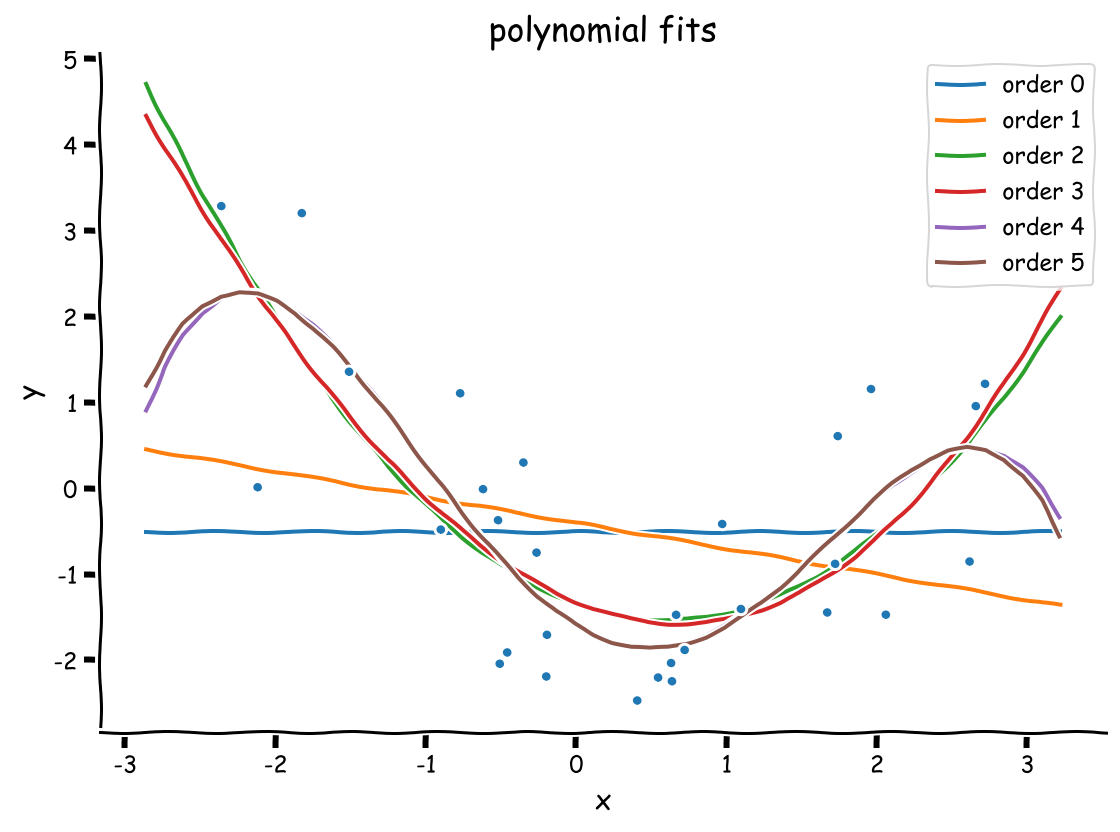
\includegraphics[scale=0.1]{Figures/ModelFitting/MFFigure4.png}
\end{subbox}
\end{textbox}
%%%%%%%%%%%%%%%%%%%%%%%%% 
%%%%%%%%%%%%%%%%%%%%%%%%%
\begin{textbox}{\href{https://compneuro.neuromatch.io/tutorials/W1D2_ModelFitting/student/W1D2_Tutorial5.html}{Model Selection: Bias-variance trade-off }  }
\begin{subbox}{subbox}{Train and Test}
\scriptsize

 The data used for the fitting procedure for a given model is the \textbf{training data}. We computed MSE on the training data of our polynomial regression models and compared training MSE across models. An additional important type of data is \textbf{test data}. This is held-out data that is not used (in any way) during the fitting procedure. When fitting models, we often want to consider both the train error (the quality of prediction on the training data) and the test error (the quality of prediction on the test data).
 
\centering
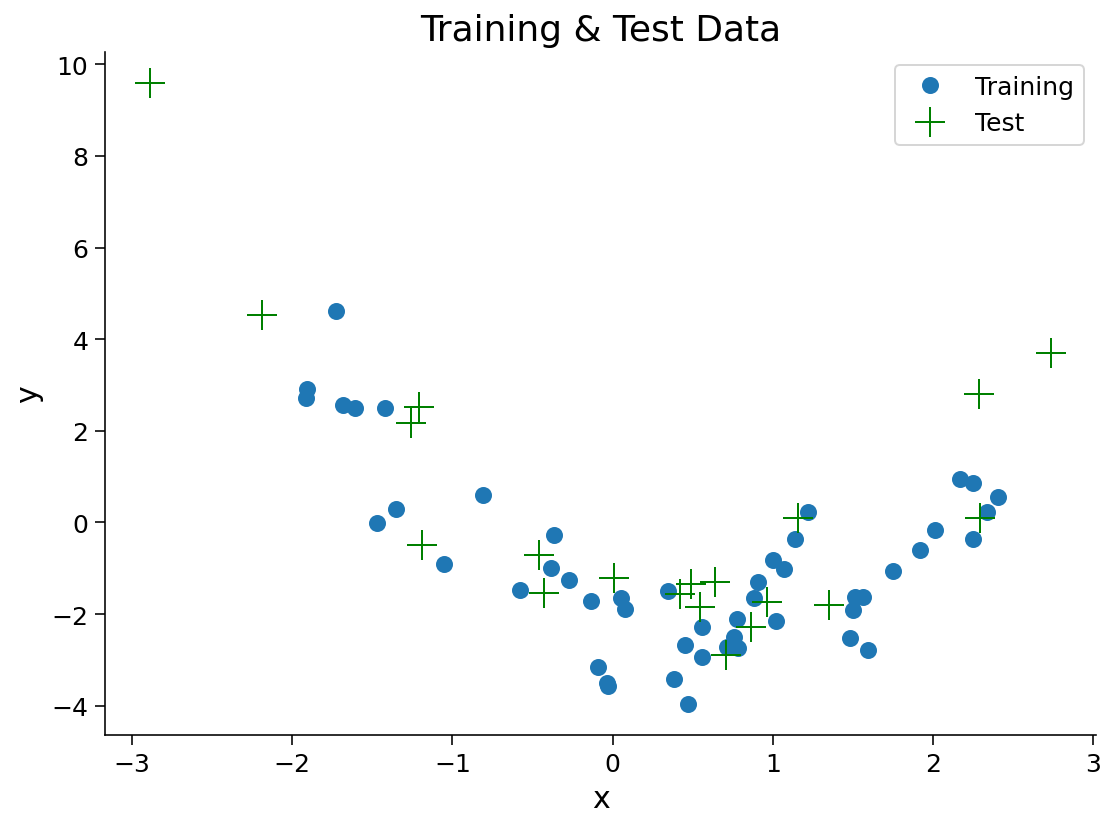
\includegraphics[scale=0.2]{Figures/ModelFitting/MFFigure5.png}
\end{subbox}
\begin{subbox}{subbox}{Bias-Variance Tradeoff}
\scriptsize
Finding a good model can be difficult. One of the most important concepts to keep in mind when modeling is the \textbf{bias-variance tradeoff}. 

\textbf{Bias} is the difference between the prediction of the model and the corresponding true output variables you are trying to predict. Models with high bias will not fit the training data well since the predictions are quite different from the true data. These high bias models are overly simplified - they do not have enough parameters and complexity to accurately capture the patterns in the data and are thus \textbf{underfitting}.


\textbf{Variance} refers to the variability of model predictions for a given input. Essentially, do the model predictions change a lot with changes in the exact training data used? Models with high variance are highly dependent on the exact training data used - they will not generalize well to test data. These high variance models are \textbf{overfitting} to the data.

\centering
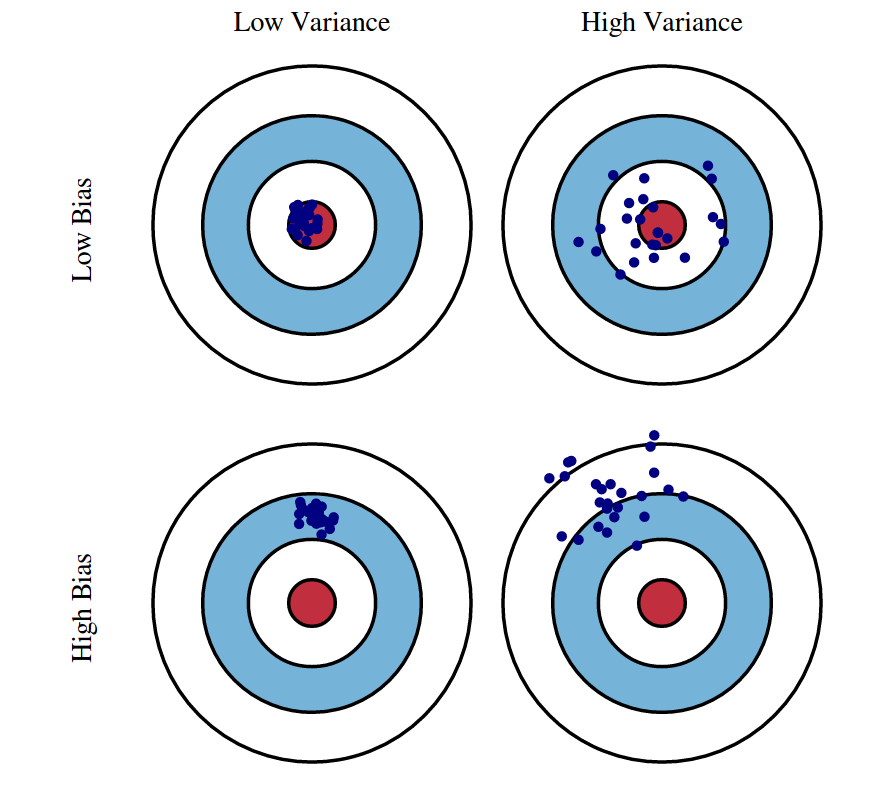
\includegraphics[scale=0.13]{Figures/ModelFitting/MFFigure6.png}
\end{subbox}
\end{textbox}
\end{multicols}
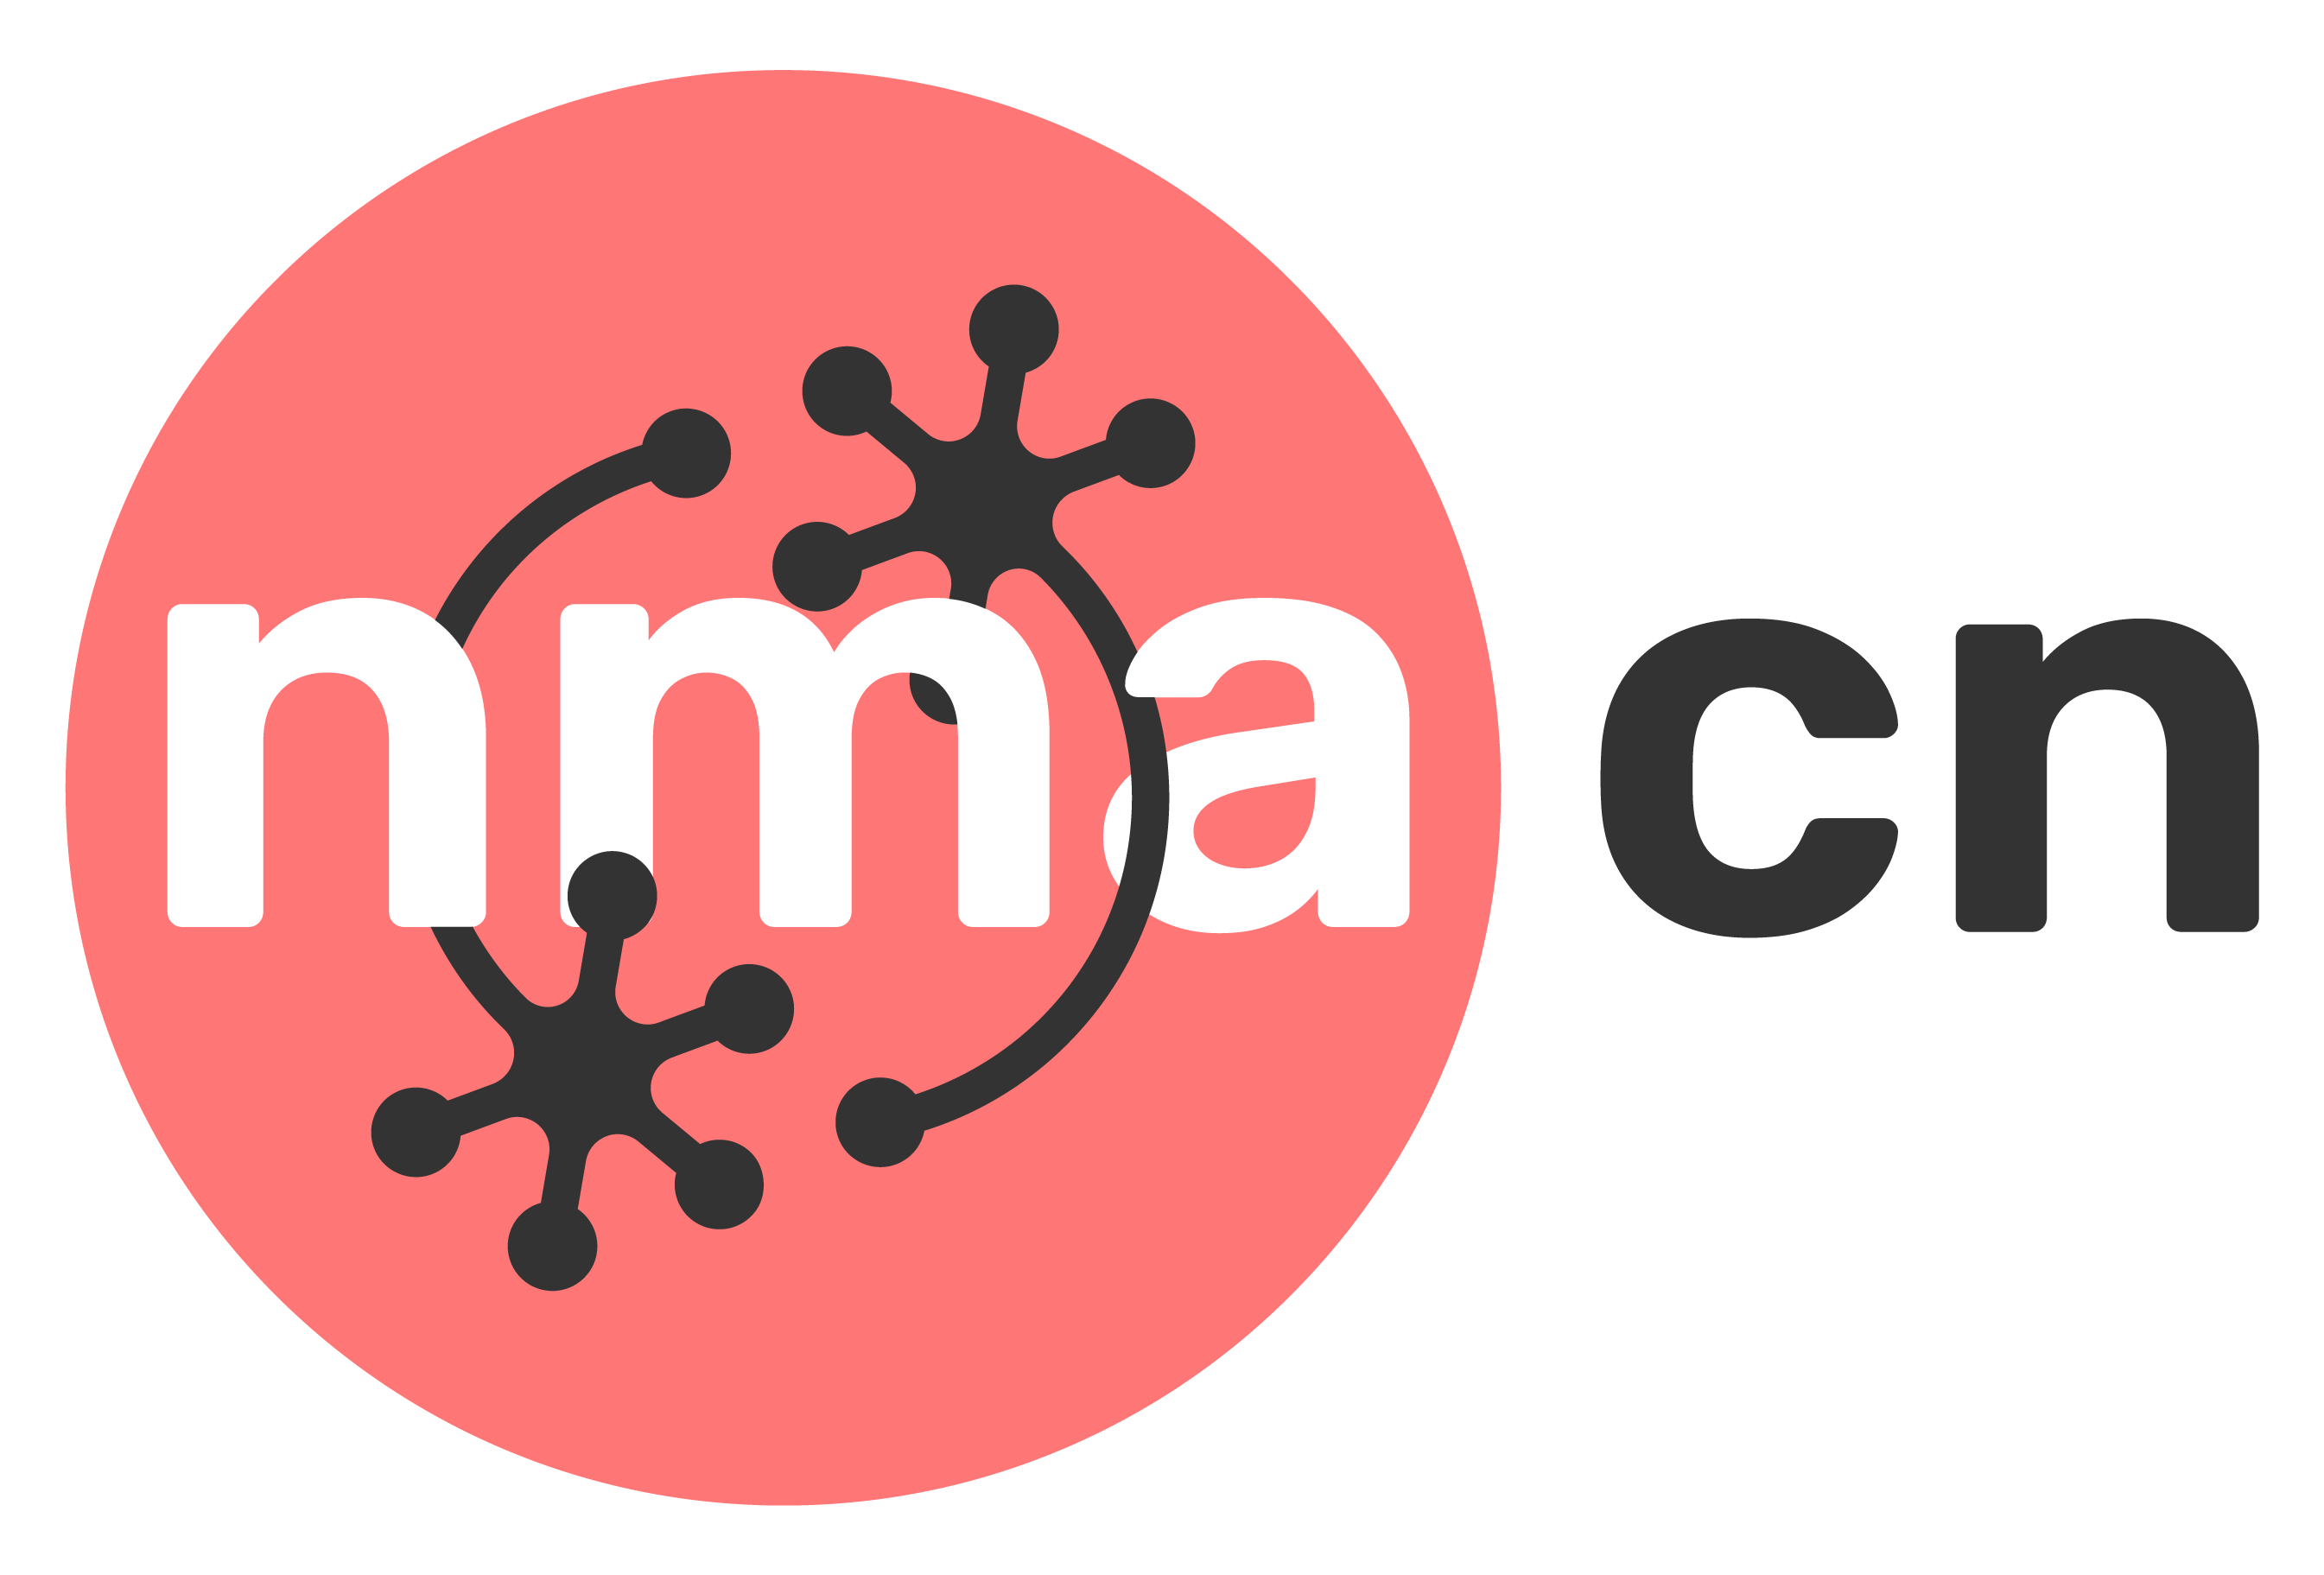
\includegraphics[scale=0.03]{Figures/NMACN.png}\href{https://compneuro.neuromatch.io/tutorials/intro.html}{\textbf{\Huge{Neuromatch Academy: Generalised Linear Models - Summary Sheet}}\footnote{’t Hart et al., (2022). Neuromatch Academy: a 3-week, online summer school in computational neuroscience. Journal of Open Source Education, 5(49), 118. https://doi.org/10.21105/jose.00118}}
\begin{multicols}{3}
\let\clearpage\relax
\begin{textbox}{\href{https://compneuro.neuromatch.io/tutorials/W1D4_GeneralizedLinearModels/student/W1D4_Tutorial1.html}{Generalized Linear Models (W1D4T1)} }
\begin{subbox}{subbox}{Create design matrix}
\scriptsize

To create the \textbf{design matrix} which organizes the stimulus intensities in matrix form such that the $i$th row has the stimulus frames preceding timepoint $i$.

In this example, we will create the design matrix $\mathbf{X}$ using $d=25$ time lags. That is, $\mathbf{X}$ should be a $T \times d$ matrix. $d = 25$  is a choice we're making based on our prior knowledge of the temporal window that influences RGC responses. 
Here, spike count is $\mathbf{Y}$ is predicted from out stimulus $\mathbf{X}$,
\centering
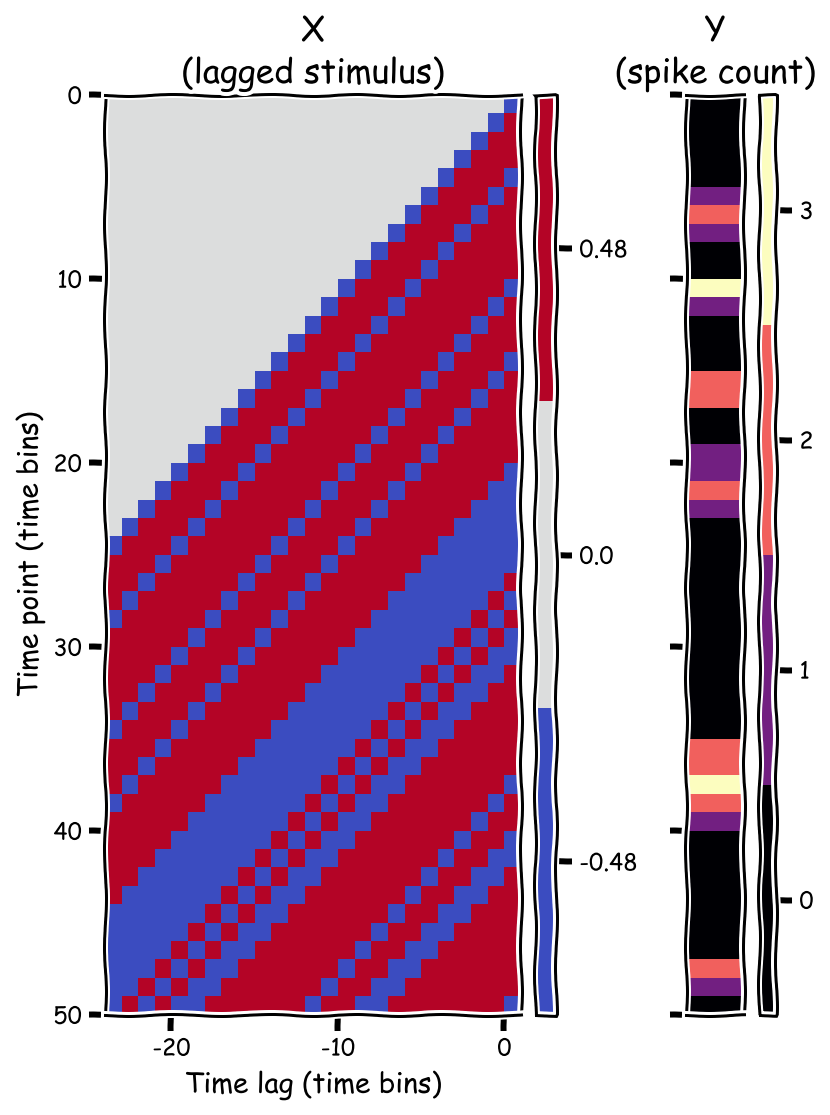
\includegraphics[scale=0.11]{Figures/GLM/GLMFigure1.png}
\end{subbox}

\begin{subbox}{subbox}{Fit Linear-Gaussian regression model 
}
\scriptsize{The maximum likelihood estimate of $\theta$ in this model can be solved analytically using the equation:

\begin{align}
\boldsymbol{\hat \theta} = (\mathbf{X}^{\top}\mathbf{X})^{-1}\mathbf{X}^{\top}\mathbf{y}.
\end{align}}
The resulting maximum likelihood filter estimates are:
\centering
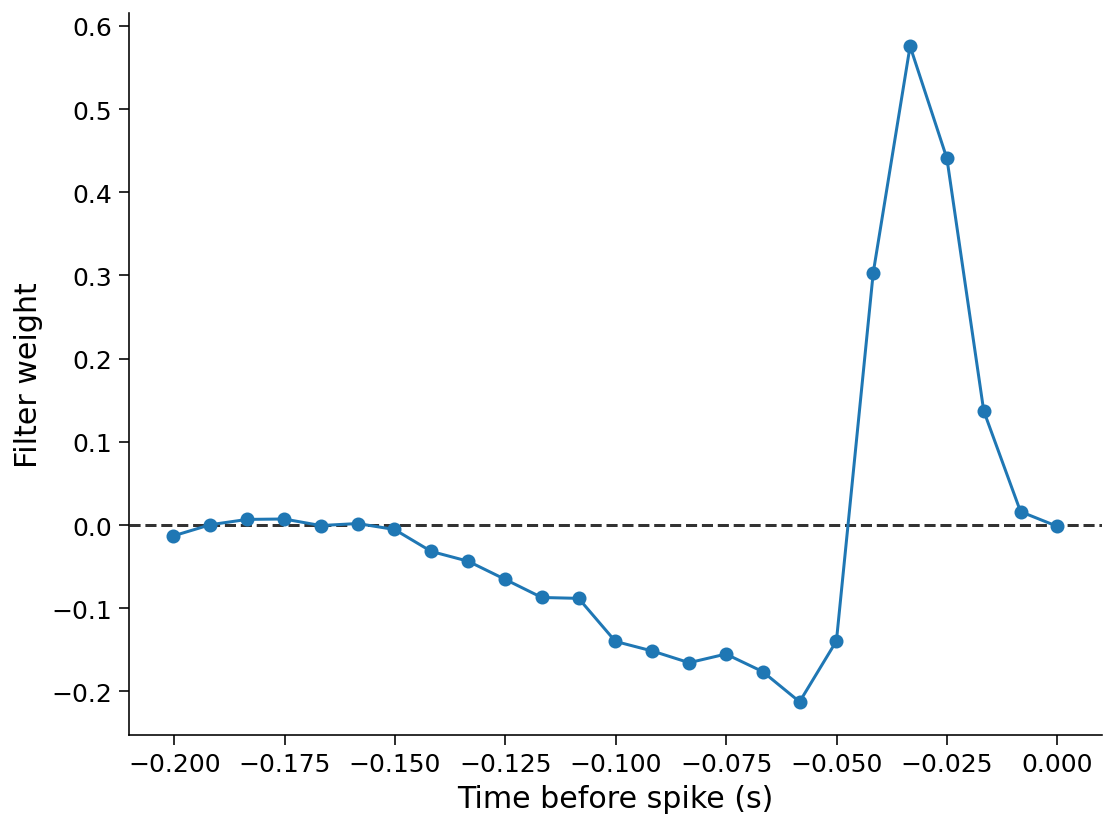
\includegraphics[scale=0.2]{Figures/GLM/GLMFigure2.png}
\end{subbox}
\end{textbox}
%%%%%%%%%%%%%%%%%%%%%%%%%%%%%%%%%%%%%%%%%%%%%%%%%%
%%%%%%%%%%%%%%%%%%%%%%%%%%%%%%%%%%%%%%%%%%%%%%%%%%
\begin{textbox}{\href{https://compneuro.neuromatch.io/tutorials/W1D4_GeneralizedLinearModels/student/W1D4_Tutorial1.html}{Generalized Linear Models (W1D4T1)} }
\begin{subbox}{subbox}{Poisson regression}
\scriptsize
Poisson regression is a generalized linear model form of regression analysis used to model count data, like spikes.
In the Poisson GLM,
\begin{align}
\log P(\mathbf{y} \mid \mathbf{X}, \theta) = \sum_t \log P(y_t \mid \mathbf{x_t},\theta),
\end{align}
where
\begin{align}
P(y_t \mid \mathbf{x_t}, \theta) = \frac{\lambda_t^{y_t}\exp(-\lambda_t)}{y_t!} \text{, with rate } \lambda_t = \exp(\mathbf{x_t}^{\top} \theta).
\end{align}

Now, taking the log likelihood for all the data we obtain:
$\log P(\mathbf{y} \mid X, \theta) = \sum_t( y_t \log\left(\lambda_t) - \lambda_t - \log(y_t !)\right).$

Because we are going to minimize the negative log likelihood with respect to the parameters $\theta$, we can ignore the last term that does not depend on $\theta$. For faster implementation, let us rewrite this in matrix notation:

\begin{align}
\mathbf{y}^{\top} \log(\mathbf{\lambda}) - \mathbf{1}^{\top} \mathbf{\lambda} \text{, with  rate } \mathbf{\lambda} = \exp(\mathbf{X} \theta)
\end{align}

Finally, don't forget to add the minus sign for your function to return the negative log likelihood.

\centering
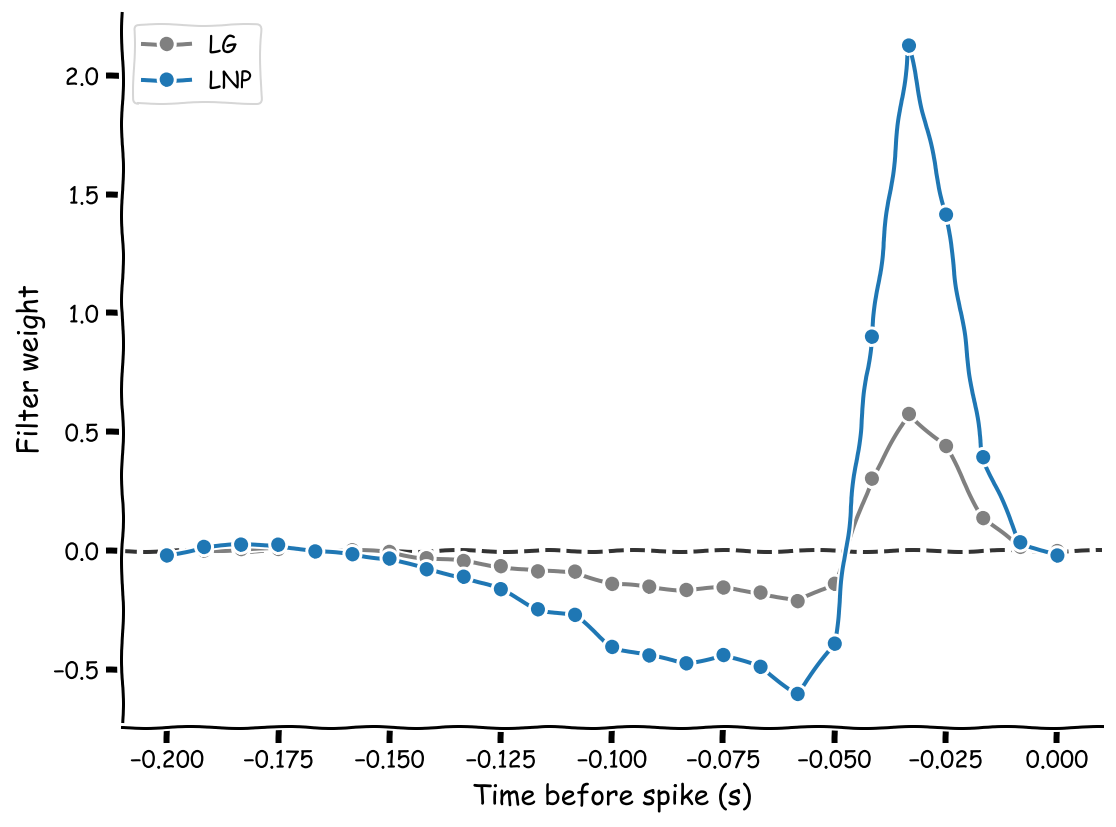
\includegraphics[scale=0.1]{Figures/GLM/GLMFigure3.png}
\end{subbox}

\begin{subbox}{subbox}{Spike Prediction 
}

\centering
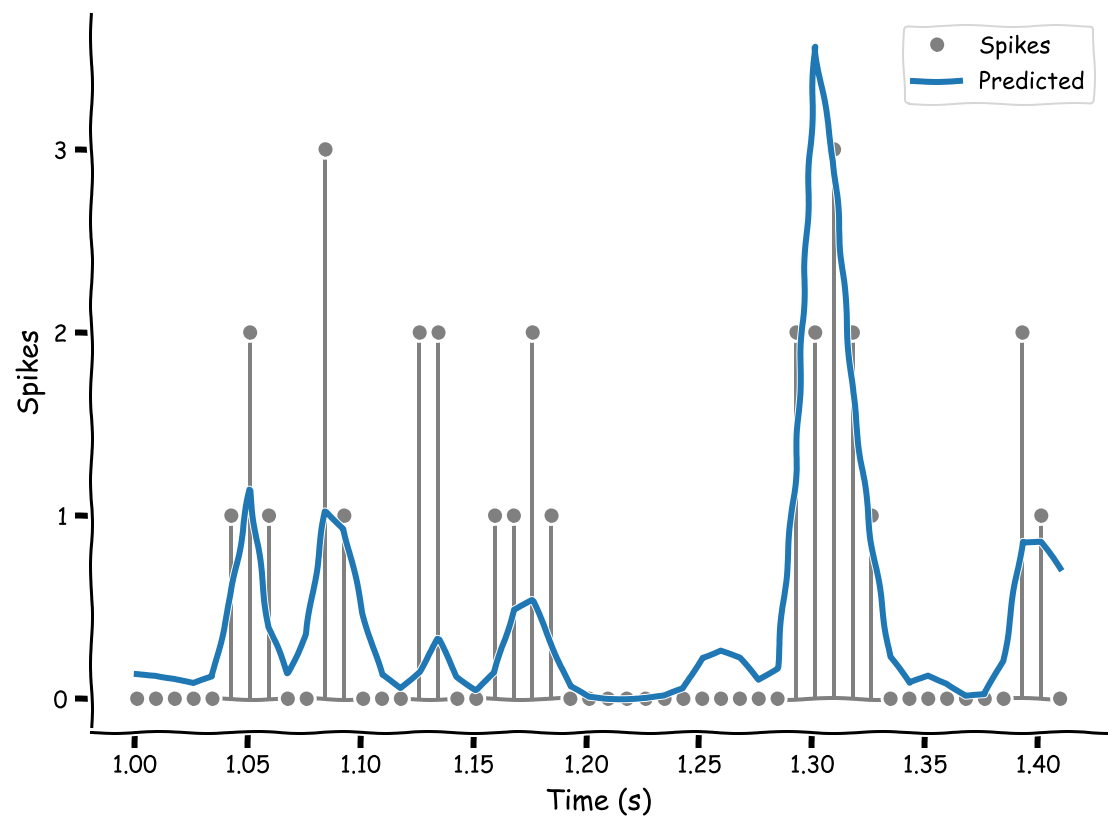
\includegraphics[scale=0.1]{Figures/GLM/GLMFigure4.png}
\end{subbox}
\end{textbox}
\begin{textbox}{\href{https://compneuro.neuromatch.io/tutorials/W1D4_GeneralizedLinearModels/student/W1D4_Tutorial2.html}{Generalized Linear Models (W1D4T2)} }
\begin{subbox}{subbox}{Logistic regression}
\scriptsize
Logistic Regression is a binary classification model. It is a GLM with a logistic link function and a Bernoulli (i.e. coinflip) noise model.
The fundamental input/output equation of logistic regression is:

\begin{align}
\hat{y} \equiv p(y=1|x,\theta) = \sigma(\theta^Tx)
\end{align}

Note that we interpret the output of logistic regression, $\hat{y}$, as the probability that $y = 1$ given inputs $x$ and parameters $\theta$.

Here $\sigma()$ is a "squashing" function called the sigmoid function or logistic function. Its output is in the range $0 \leq y \leq 1$. It looks like this:

\begin{align}
\sigma(z) = \frac{1}{1 + \textrm{exp}(-z)}
\end{align}
Recall that $z = \theta^T x$. The parameters decide whether $\theta^T x$ will be very negative, in which case $\sigma(\theta^T x)\approx 0$, or very positive, meaning  $\sigma(\theta^T x)\approx 1$.

\centering
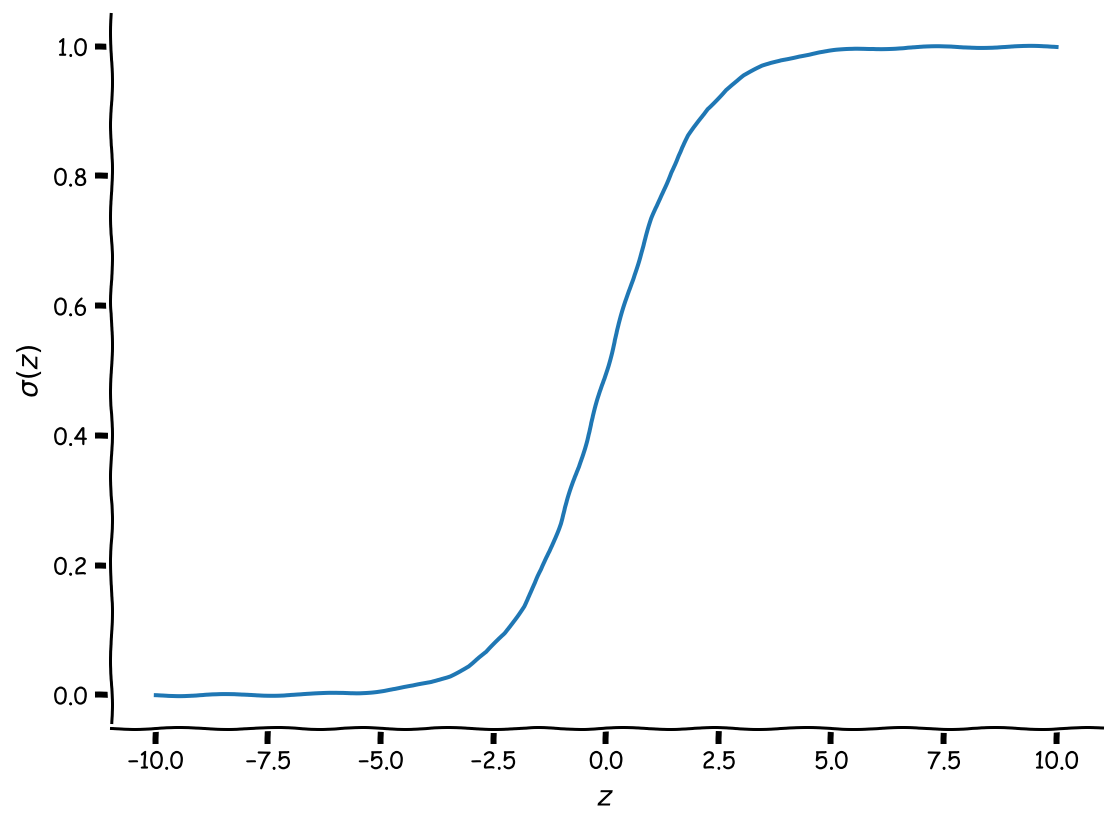
\includegraphics[scale=0.07]{Figures/GLM/GLMFigure5.png}
\end{subbox}

\begin{subbox}{subbox}{Regularisation 
}
\scriptsize
Regularization forces a model to learn a set solutions you a priori believe to be more correct, which reduces over-fitting because it doesn't have as much flexibility to fit idiosyncrasies in the training data. This adds model bias, but it's a good bias because you know (maybe) that parameters should be small or mostly 0.

\textbf{$L_2$ regularization}\\
Regularization comes in different flavors. A very common one uses an $L_2$ or "ridge" penalty. This changes the objective function to
\begin{align}
-\log\mathcal{L}'(\theta | X, y)=
-\log\mathcal{L}(\theta | X, y) +\frac\beta2\sum_i\theta_i^2,
\end{align}
where $\beta$ is a \textit{hyperparameter} that sets the \textit{strength} of the regularization.

\end{subbox}
\end{textbox}
\end{multicols}
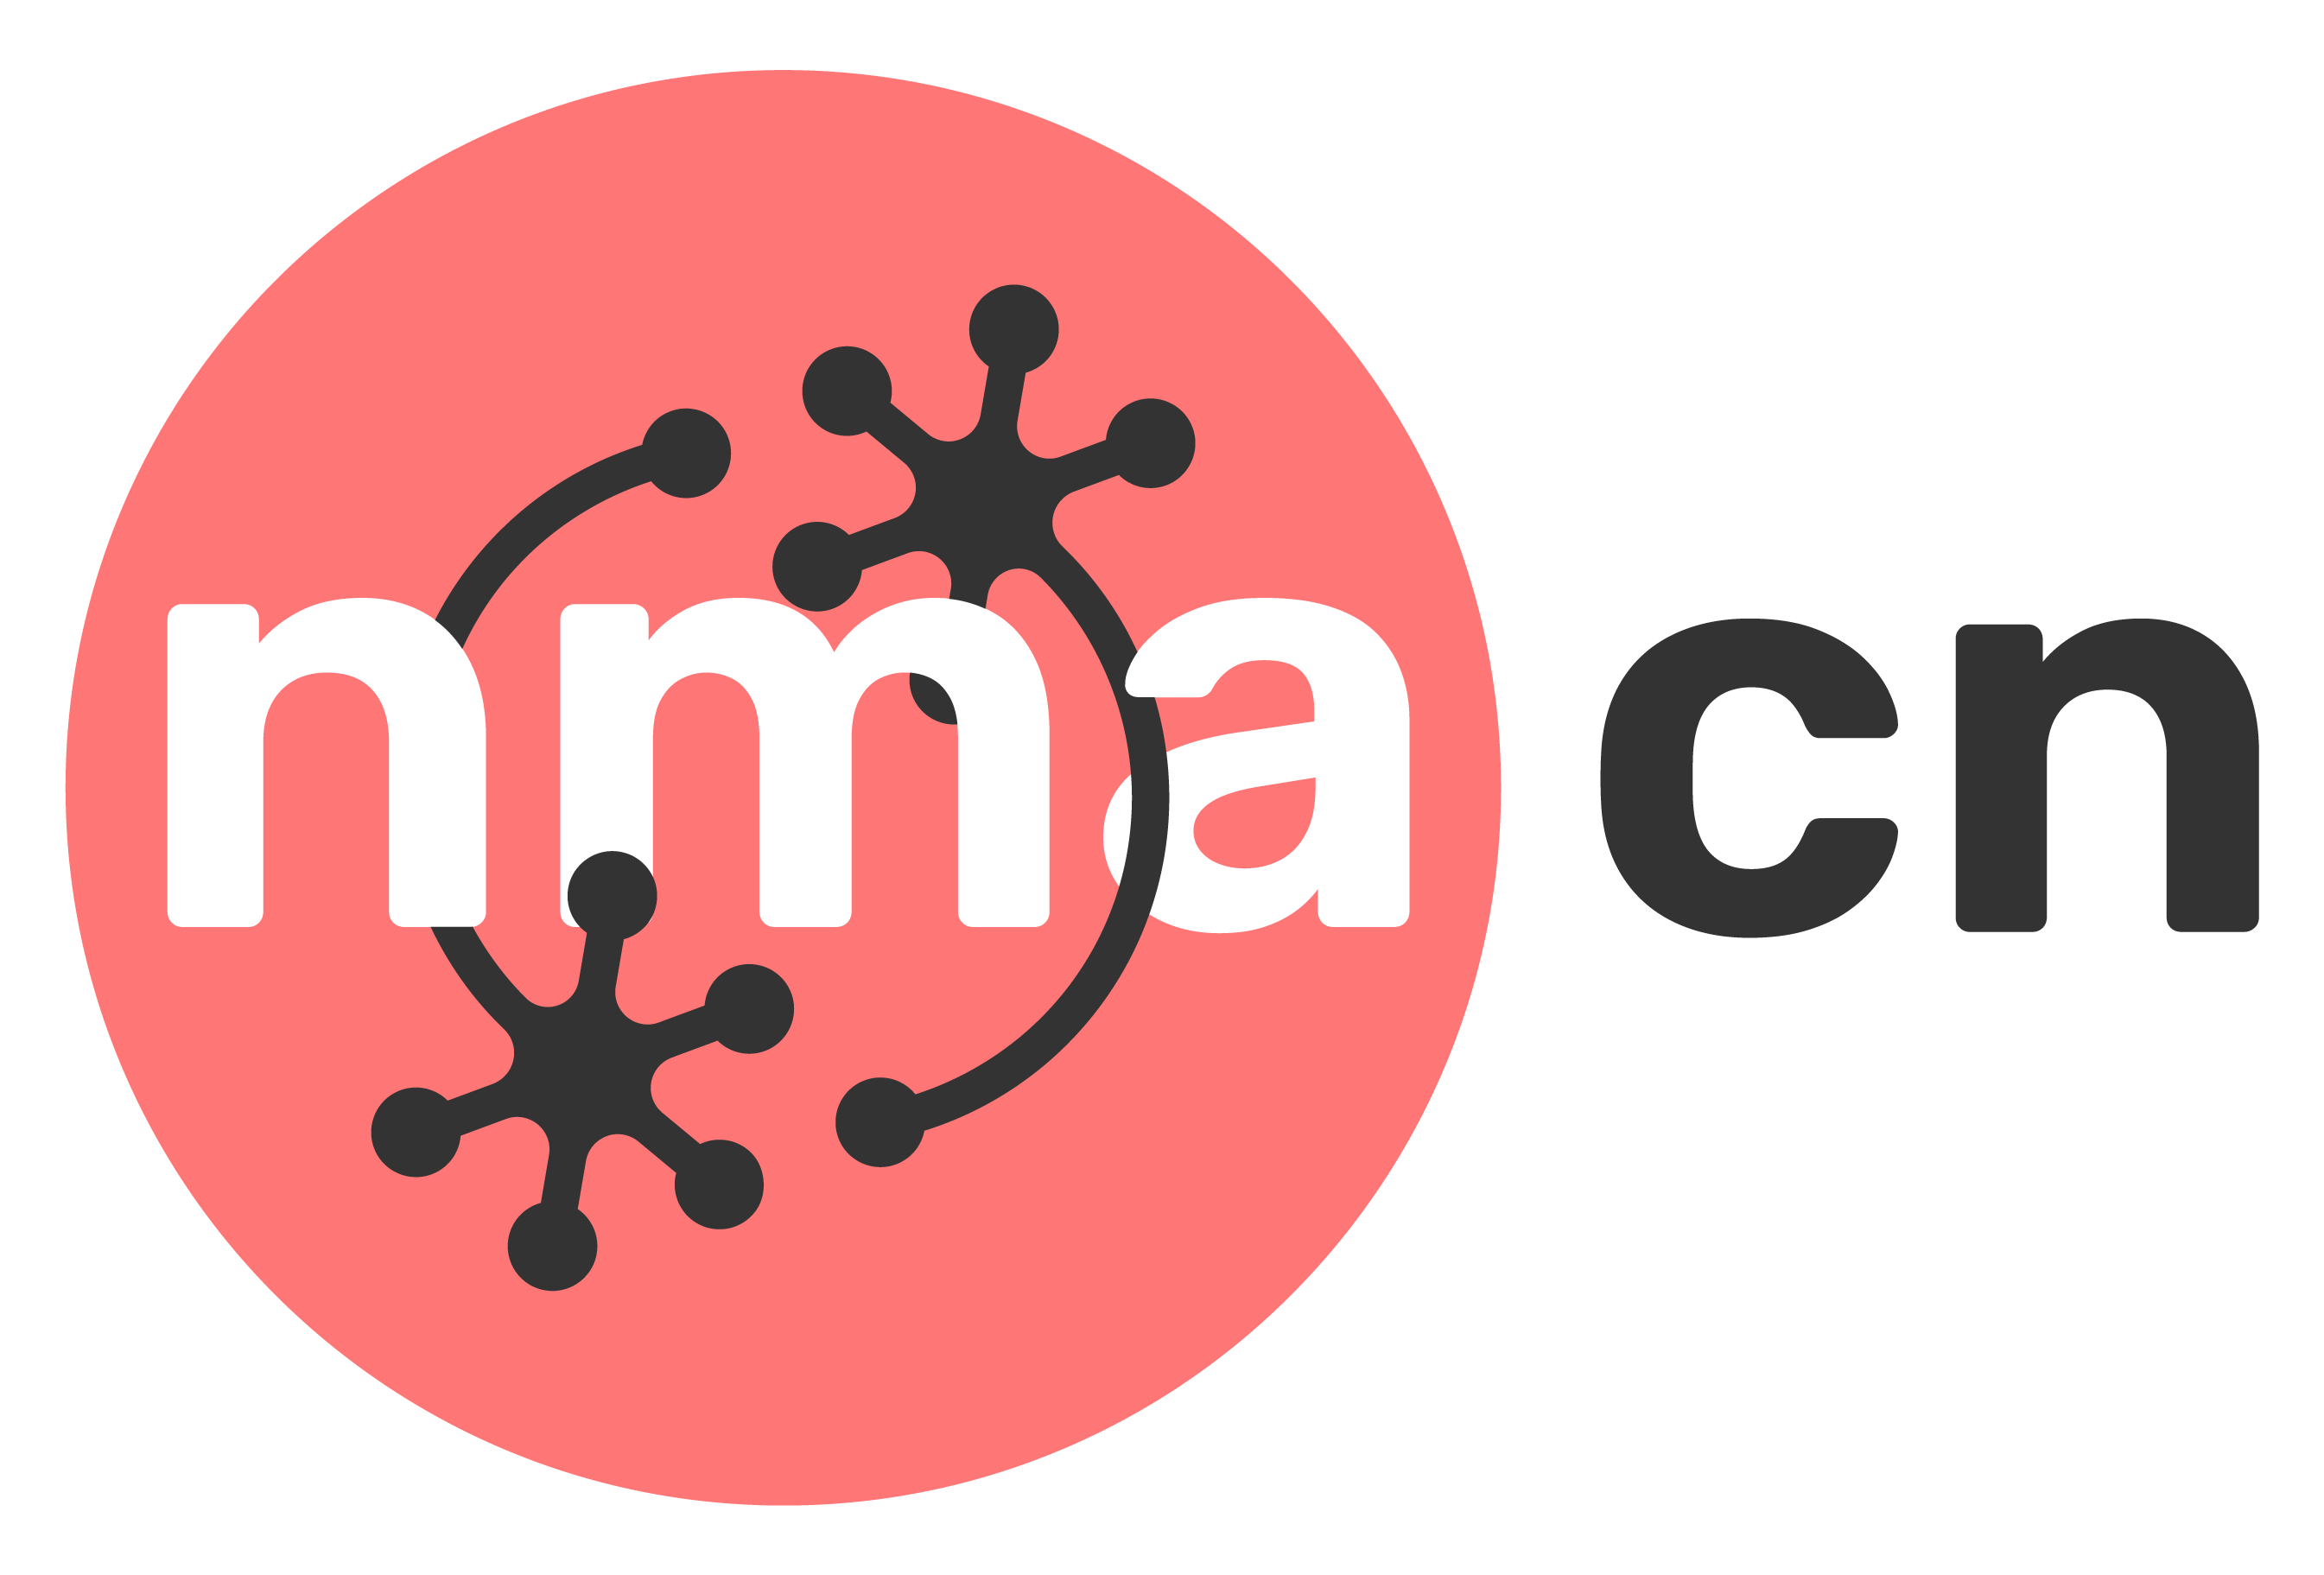
\includegraphics[scale=0.03]{Figures/NMACN.png}\href{https://compneuro.neuromatch.io/tutorials/intro.html}{\textbf{\Huge{Neuromatch Academy: Dimensionality Reduction - Summary\\ Sheet }}\footnote{’t Hart et al., (2022). Neuromatch Academy: a 3-week, online summer school in computational neuroscience. Journal of Open Source Education, 5(49), 118. https://doi.org/10.21105/jose.00118}}
\begin{multicols}{3}
\let\clearpage\relax

\begin{textbox}{\href{https://compneuro.neuromatch.io/tutorials/W1D5_DimensionalityReduction/student/W1D5_Tutorial1.html}{Dimensionality Reduction (W1D5T1)} }
\begin{subbox}{subbox}{Generate Correlated Multivariate Data}
\scriptsize
 Multivariate data can be visualized as a cloud of points in a high-dimensional vector space. The geometry of this cloud is shaped by the covariance matrix.

The covariance can be found from the equation above:

\begin{align}
\text{cov}(x_1,x_2) = \rho \sqrt{\sigma_1^2 \sigma_2^2}.
\end{align}
The covariance matrix for two dimensions has the following form:

\begin{align}
{\bf \Sigma} = 
\begin{pmatrix}
 \text{var}(x_1) & \text{cov}(x_1,x_2) \\
 \text{cov}(x_1,x_2) &\text{var}(x_2)
\end{pmatrix}.
\end{align}

\centering
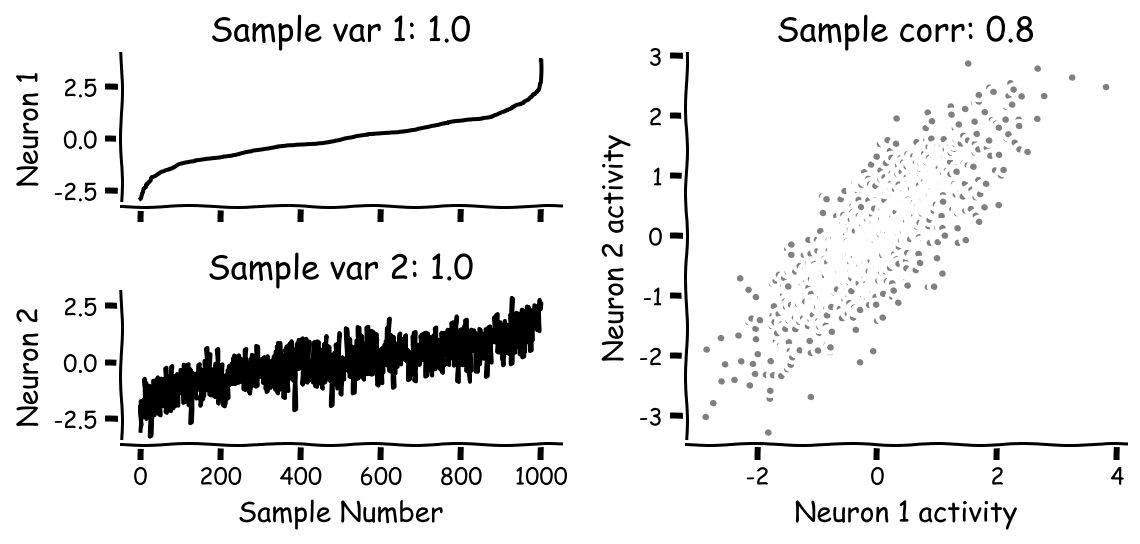
\includegraphics[scale=0.15]{Figures/DM/DMFigure1.png}
\end{subbox}

\begin{subbox}{subbox}{Orthonormal Basis
}
\scriptsize
Two vectors are orthonormal if: 
\begin{enumerate}
    \item 
   They are orthogonal (i.e., their dot product is zero):
\begin{align}
{\bf u\cdot w} = u_1 w_1 + u_2 w_2 = 0
\end{align}
\item   They have unit length:
\begin{align}
||{\bf u} || = ||{\bf w} || = 1
\end{align}
\end{enumerate}
\centering
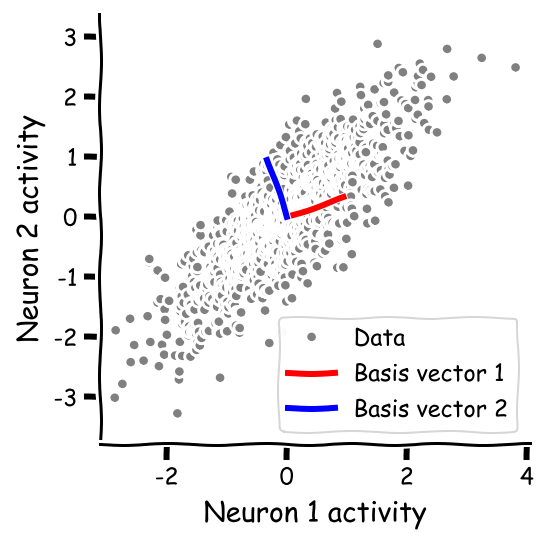
\includegraphics[scale=0.18]{Figures/DM/DMFigure2.png}

\end{subbox}
\end{textbox}
%%%%%%%%%%%%%%%%%%%%%%%%%%%%%%%%%%%%%%%%%%%%%%%%%%%%%%%
%%%%%%%%%%%%%%%%%%%%%%%%%%%%%%%%%%%%%%%%%%%%%%%%%%%%%%%
\begin{textbox}{\href{https://compneuro.neuromatch.io/tutorials/W1D5_DimensionalityReduction/student/W1D5_Tutorial2.html}{Principal Component Analysis (W1D5T2)} }
\begin{subbox}{subbox}{Eigenvectors of the Sample Covariance Matrix}
\scriptsize
PCA represents data in a new orthonormal basis defined by the eigenvectors of the covariance matrix. The bivariate normal data with a specified covariance matrix $\bf \Sigma$, whose $(i,j)$th element is:
\begin{align}
\Sigma_{ij} = \mathbb{E}[ x_i x_j ] - \mathbb{E}[ x_i] \mathbb{E}[ x_j ] .
\end{align}
 We use the sample covariance matrix, $\bf\hat\Sigma$, which is calculated directly from the data. The $(i,j)$th element of the sample covariance matrix is:
\begin{align}
 \hat \Sigma_{ij} =  \frac{1}{N_\text{samples}}{\bf x}_i^T {\bf x}_j - \bar {\bf x}_i \bar{\bf x}_j ,
\end{align}
where ${\bf x}_i = [ x_i(1), x_i(2), \dots,x_i(N_\text{samples})]^T$ is a column vector representing all measurements of neuron $i$, and  $\bar {\bf x}_i$ is the mean of neuron $i$ across samples:
\begin{align}
\bar {\bf x}_i = \frac{1}{N_\text{samples}} \sum_{k=1}^{N_\text{samples}} x_i(k).
\end{align}
If we assume that the data has already been mean-subtracted, then we can write the sample covariance matrix in a much simpler matrix form:
\begin{align}
{\bf \hat \Sigma}
&= \frac{1}{N_\text{samples}} {\bf X}^T {\bf X}.
\end{align}

where $\bf X$ is the full data matrix (each column of $\bf X$ is a different $\bf x_i$). 
\end{subbox}

\end{textbox}
%%%%%%%%%%%%%%%%%%%%%%%%%%%%%%%%%%%%%%%%%%%%%%%%%%%%%
%%%%%%%%%%%%%%%%%%%%%%%%%%%%%%%%%%%%%%%%%%%%%%%%%%%%%
\begin{textbox}{\href{https://compneuro.neuromatch.io/tutorials/W1D5_DimensionalityReduction/student/W1D5_Tutorial2.html}{Principal Component Analysis (W1D5T2)} }

\begin{subbox}{subbox}{PCA by projecting data onto the eigenvectors
}
\scriptsize
To perform PCA project the data onto the eigenvectors of the covariance matrix, i.e.:
\begin{align}
\bf S = X W
\end{align}
where $\bf S$ is an $N_\text{samples} \times N$ matrix representing the projected data (also called \textit{scores}), and $\bf W$ is an $N\times N$ orthogonal matrix, each of whose columns represents the eigenvectors of the covariance matrix (also called \textit{weights} or \textit{loadings}). 
Since $\bf W$ is an orthogonal matrix, ${\bf W}^{-1} = {\bf W}^T$. So by multiplying by ${\bf W}^T$ on each side we can rewrite this equation as  
\begin{align}
{\bf X = S W}^T.
\end{align}
To reconstruct the data from a low-dimensional approximation, we just have to truncate these matrices.  Let's denote ${\bf S}_{1:K}$ and ${\bf W}_{1:K}$ the matrices with only the first $K$ columns of $\bf S$ and $\bf W$, respectively. Then our reconstruction is:
\begin{align}
{\bf \hat X = S}_{1:K} ({\bf W}_{1:K})^T.
\end{align}
\end{subbox}
\end{textbox}
%%%%%%%%%%%%%%%%%%%%%%%%%%%%%%%%%%%%%%%%%%%%%%%%%%%%%
%%%%%%%%%%%%%%%%%%%%%%%%%%%%%%%%%%%%%%%%%%%%%%%%%%%%%
\begin{textbox}{\href{https://compneuro.neuromatch.io/tutorials/W1D5_DimensionalityReduction/student/W1D5_Tutorial3.html}{Dimensionality Reduction \& Reconstruction (W1D5T3)} }
\begin{subbox}{subbox}{Scree Plot}
\scriptsize

Each eigenvalue describes the variance of the data projected onto its corresponding eigenvector. This is an important concept because it allows us to rank the PCA basis vectors based on how much variance each one can capture in a scree plot.
A scree plot is used to help choose which and how many components to use:
\centering
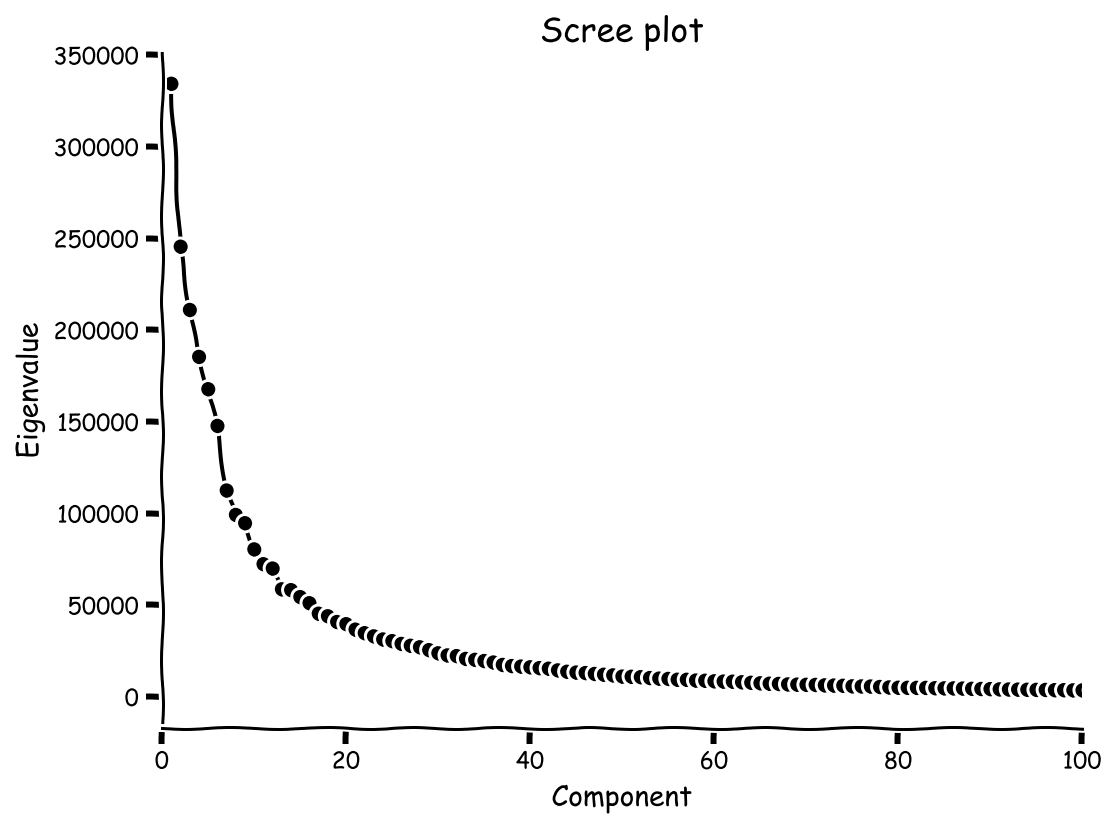
\includegraphics[scale=0.13]{Figures/DM/DMFigure3.png}

\end{subbox}

\begin{subbox}{subbox}{Calculate the variance explained
}
\scriptsize
Another common way to determine the intrinsic dimensionality is by considering the variance explained. This can be examined with a cumulative plot of the fraction of the total variance explained by the top $K$ components, i.e.,
\begin{align}
\text{var explained} = \frac{\sum_{i=1}^K \lambda_i}{\sum_{i=1}^N \lambda_i}
\end{align}
where $\lambda_i$ is the $i^{th}$ eigenvalue and $N$ is the total number of components (the original number of dimensions in the data).
The intrinsic dimensionality is often quantified by the $K$ necessary to explain a large proportion of the total variance of the data (often a defined threshold, e.g., 90\%).

\centering
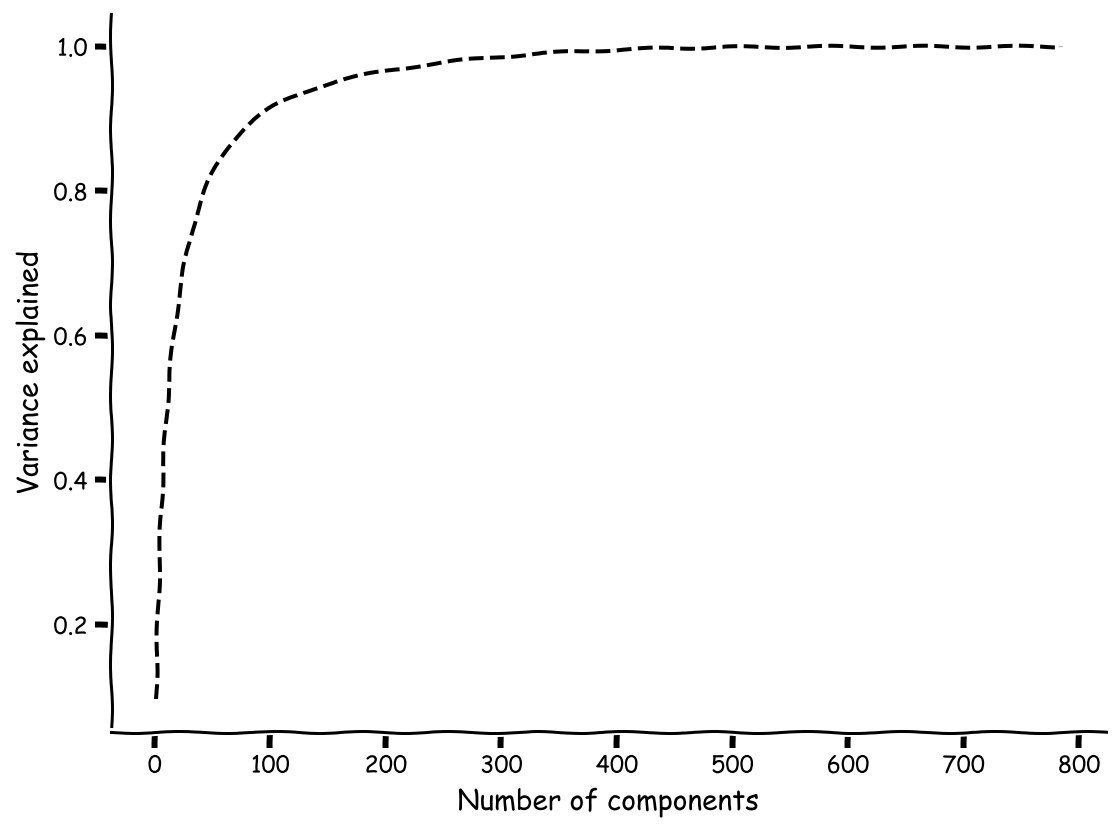
\includegraphics[scale=0.15]{Figures/DM/DMFigure4.png}

\end{subbox}

\end{textbox}
%%%%%%%%%%%%%%%%%%%%%%%%%%%%%%%%%%%%%%%%%%%%%%%%%%%%
%%%%%%%%%%%%%%%%%%%%%%%%%%%%%%%%%%%%%%%%%%%%%%%%%%%%
\begin{textbox}{\href{https://compneuro.neuromatch.io/tutorials/W1D5_DimensionalityReduction/student/W1D5_Tutorial4.html}{ Nonlinear Dimensionality Reduction (W1D5T4)} }
\begin{subbox}{subbox}{Unsupervised Reduction}
\scriptsize

PCA and t-SNE are unsupervised non-linear dimensionality  reduction methods.
Nonlinear methods can be more powerful, they can also be sensitive to noise. In contrast, linear methods are useful for their simplicity and robustness.
Comparing PCA and t-SNE for data visualization. Using t-SNE, we could visualize clusters in the data corresponding to different digits. While PCA was able to separate some clusters (e.g., 0 vs 1), it performed poorly overall.
However, the results of t-SNE can change depending on the choice of perplexity.
\end{subbox}
\begin{subbox}{subbox}{Visualize MNIST in 2D using PCA}
\scriptsize

\centering
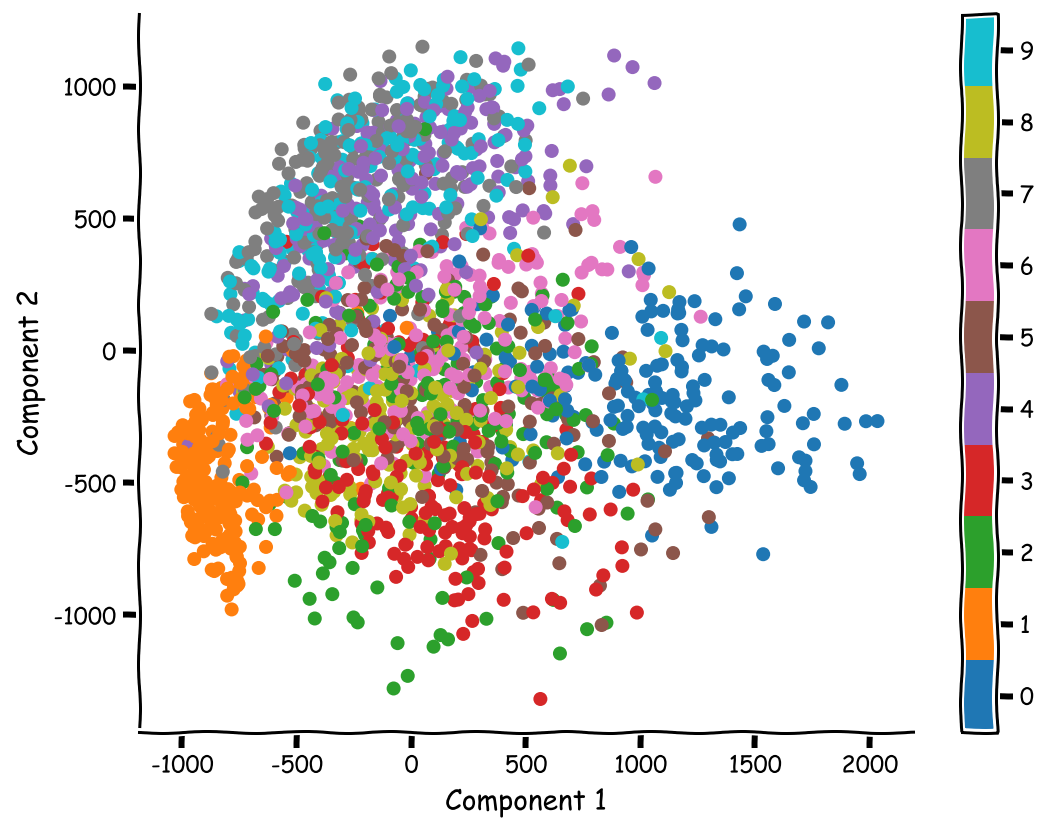
\includegraphics[scale=0.15]{Figures/DM/DMFigure5.png}

\end{subbox}
\begin{subbox}{subbox}{Visualize MNIST in 2D using t-SNE}
\scriptsize

\centering
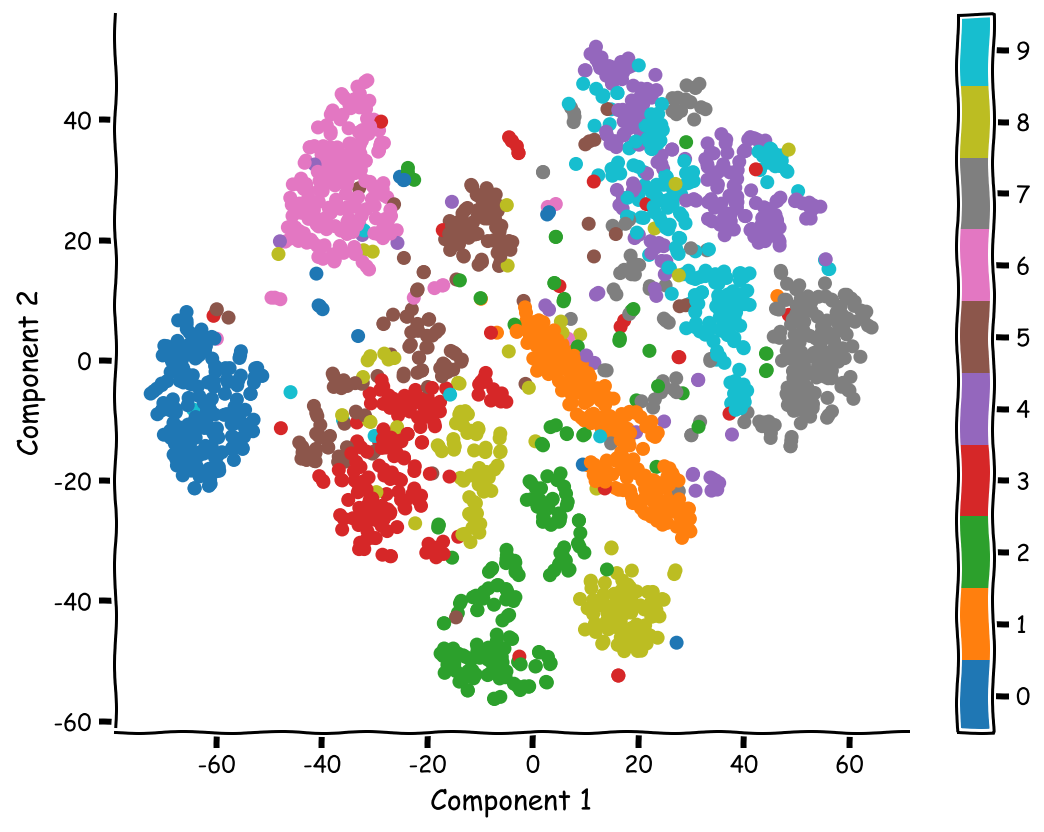
\includegraphics[scale=0.15]{Figures/DM/DMFigure6.png}

\end{subbox}

\end{textbox}
\end{multicols}
\newpage
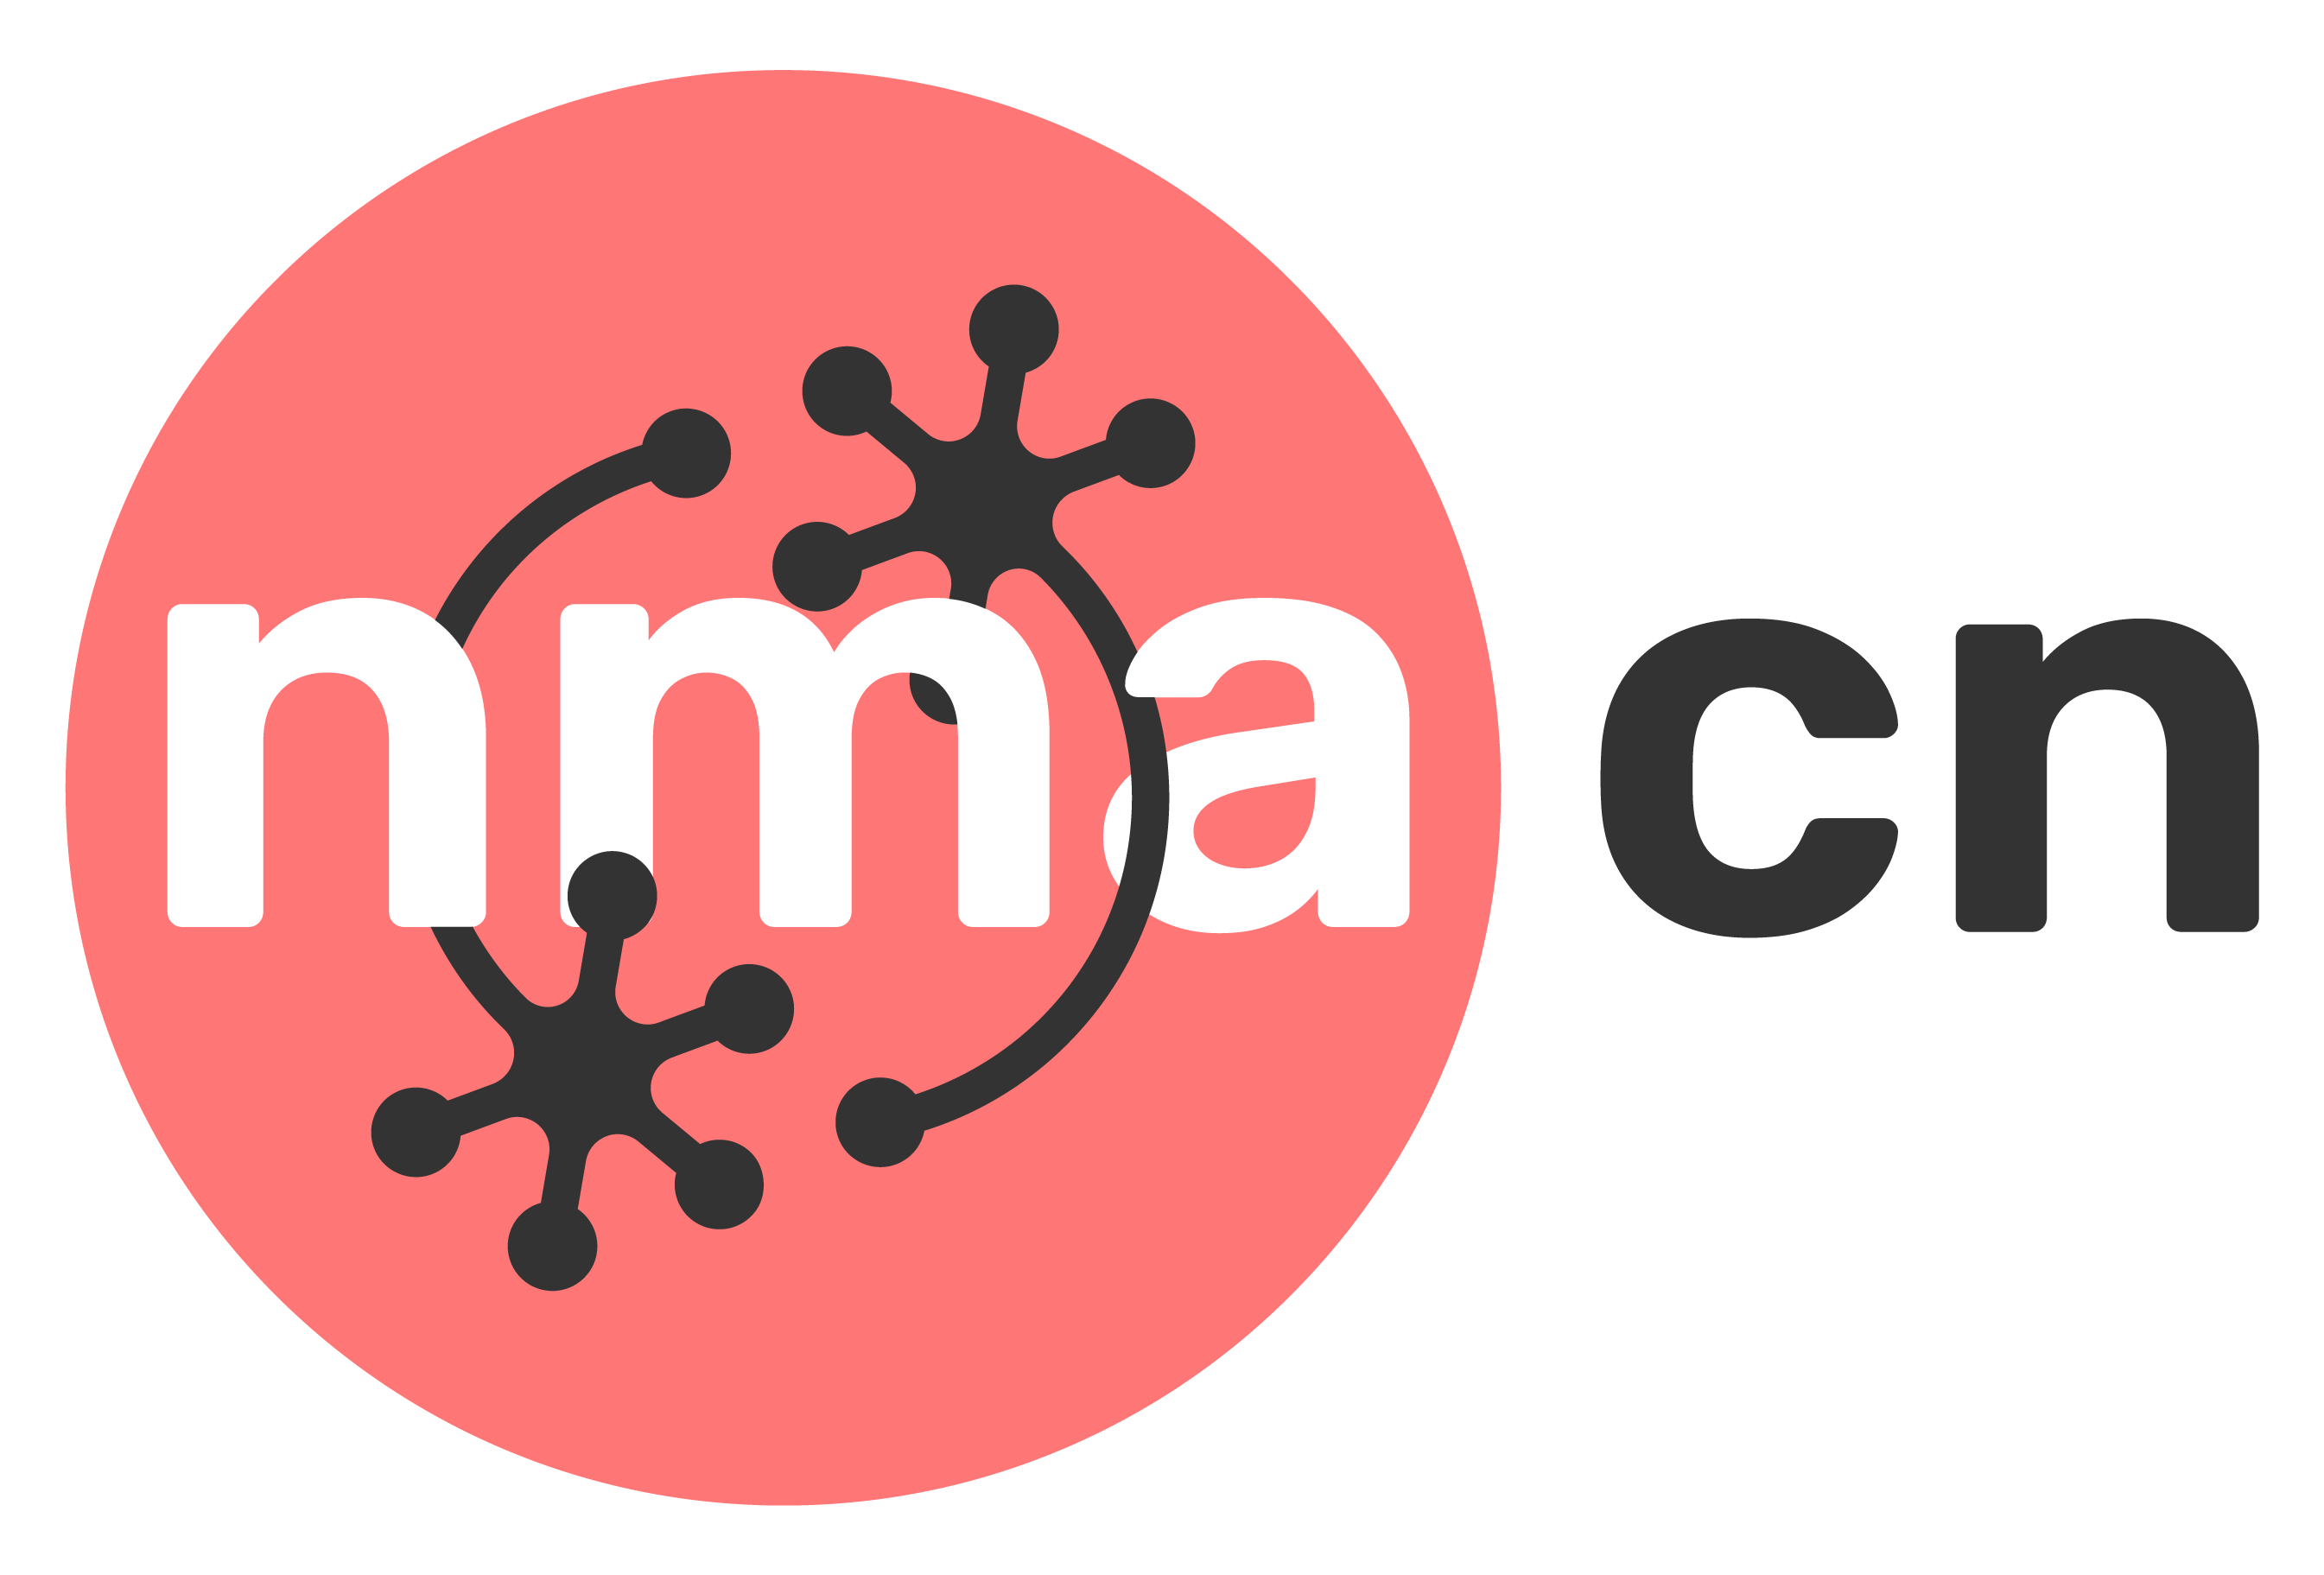
\includegraphics[scale=0.03]{Figures/NMACN.png}\href{https://compneuro.neuromatch.io/tutorials/intro.html}{\textbf{\Huge{Neuromatch Academy: Deep Learning - Summary Sheet}}\footnote{’t Hart et al., (2022). Neuromatch Academy: a 3-week, online summer school in computational neuroscience. Journal of Open Source Education, 5(49), 118. https://doi.org/10.21105/jose.00118}}
\begin{multicols}{3}
\begin{textbox}{\href{https://compneuro.neuromatch.io/tutorials/W2D1_DeepLearning/student/W2D1_Tutorial1.html}{Neural Network (W2D1T1)} }
\begin{subbox}{subbox}{Deep feed-forward networks}
\scriptsize
We can build a linear network with no hidden layers, where the stimulus prediction $y$ is a product of weights $\mathbf{W}_{out}$ and neural responses $\mathbf{r}$ with an added term $\mathbf{b}$ which is called the bias term. When you fit a linear model such as this you minimize the squared error between the predicted stimulus $y$ and the true stimulus $\tilde{y}$, this is the “loss function”. 
\begin{align}
    L &= (y - \tilde{y})^2 \\
     &= ((\mathbf{W}^{out} \mathbf{r} + \mathbf{b}) - \tilde{y})^2
\end{align}
The solution to minimizing this loss function in a linear model can be found in closed form. If we use a simple linear model for this data we are able to predict the stimulus within 2-3 degrees. 

Let’s add a hidden layer with $M$ units to this linear model, where now the output $y$ is as follows:
\begin{align}
    \mathbf{h} &= \mathbf{W}^{in} \mathbf{r} + \mathbf{b}^{in}, && [\mathbf{W}^{in}: M \times N,\, \mathbf{b}^{in}: M \times 1], \\
    y &= \mathbf{W}^{out} \mathbf{h} + \mathbf{b}^{out},  && [\mathbf{W}^{out}: 1 \times M,\, \mathbf{b}^{in}: 1 \times 1],
\end{align}

The $M$-dimensional vector $\mathbf{h}$ denotes the activations of the \textit{hidden layer} of the network. The blue components of this diagram denote the \textit{parameters} of the network, which we will later optimize with gradient descent. These include all the weights and biases $\mathbf{W}^{in}, \mathbf{b}^{in}, \mathbf{W}^{out}, \mathbf{b}^{out}$. The \textit{weights} are matrices of size (# of outputs, # of inputs) that are multiplied by the input of each layer, like the regression coefficients in linear regression.

\centering
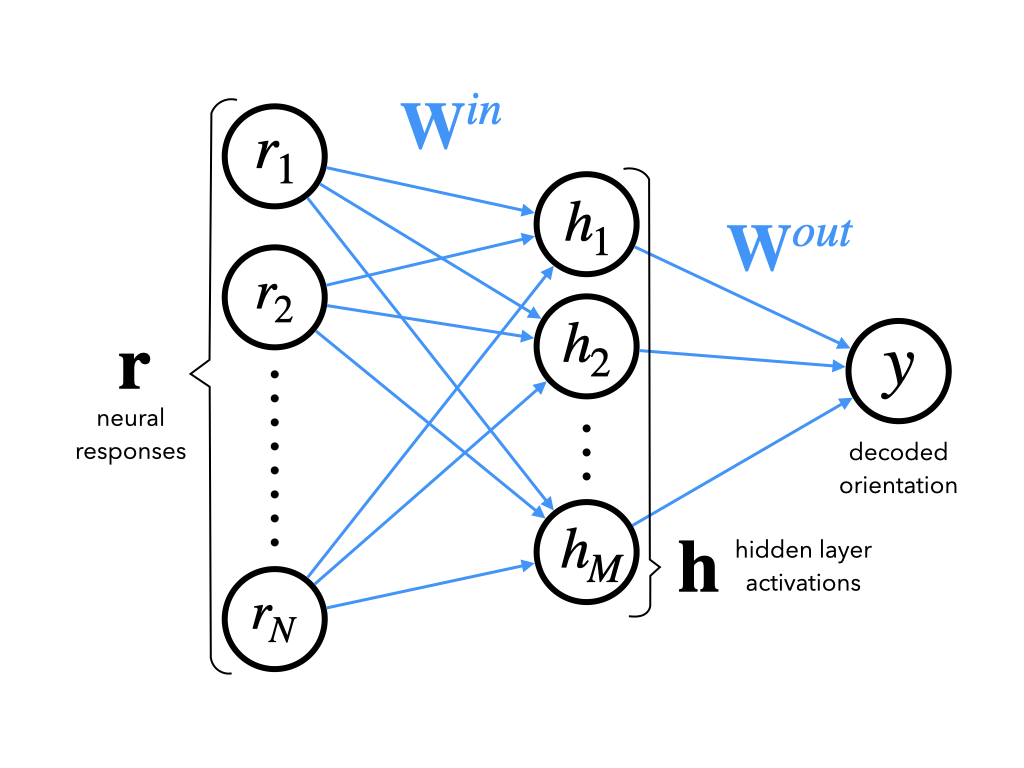
\includegraphics[scale=0.1]{Figures/DL/DLFigure1.png}
\end{subbox}


\end{textbox}
%%%%%%%%%%%%%%%%%%%%%%%%%%%%%%%%%%%%%%%%%%%%%%%%%%%%%%%
%%%%%%%%%%%%%%%%%%%%%%%%%%%%%%%%%%%%%%%%%%%%%%%%%%%%%%%
\begin{textbox}{\href{https://compneuro.neuromatch.io/tutorials/W2D1_DeepLearning/student/W2D1_Tutorial1.html}{Neural Network (W2D1T1)} }
\begin{subbox}{subbox}{Activation Functions}
\scriptsize
To extend the set of computable input/output transformations to more than just weighted sums, we'll incorporate a non-linear activation function in the hidden units. This is done by simply modifying the equation for the hidden layer activations to be
\begin{equation}
    \mathbf{h}^{(n)} = \phi(\mathbf{W}^{in} \mathbf{r}^{(n)} + \mathbf{b}^{in})
\end{equation}
where $\phi$ is referred to as the activation function. Using a non-linear activation function will ensure that the hidden layer performs a non-linear transformation of the input, which will make our network much more powerful. In practice, deep networks always use non-linear activation functions.
The most common non-linearity used is the rectified linear unit (or ReLU), which is a max(0, x) function.

\end{subbox}
\begin{subbox}{subbox}{Gradient Descent}
\scriptsize
In gradient descent we compute the gradient of the loss function with respect to each parameter (all W’s and b’s). We then update the parameters by subtracting the learning rate times the gradient. 

Let’s visualize this loss function $L$ with respect to a weight $w$. If the gradient is positive (the slope $\frac{dL}{dw}$ > 0) as in this case then we want to move in the opposite direction which is negative. So we update the $w$ accordingly in the negative direction on each iteration. Once the iterations complete the weight will ideally be at a value that minimizes the cost function.

In reality these cost functions are not convex like this one and depend on hundreds of thousands of parameters. There are tricks to help navigate this rocky cost landscape such as adding momentum or changing the optimizer but we won’t have time to get into that today. There are also ways to change the architecture of the network to improve optimization, such as including skip connections. These skip connections are used in residual networks and allow for the optimization of many layer networks.

\centering
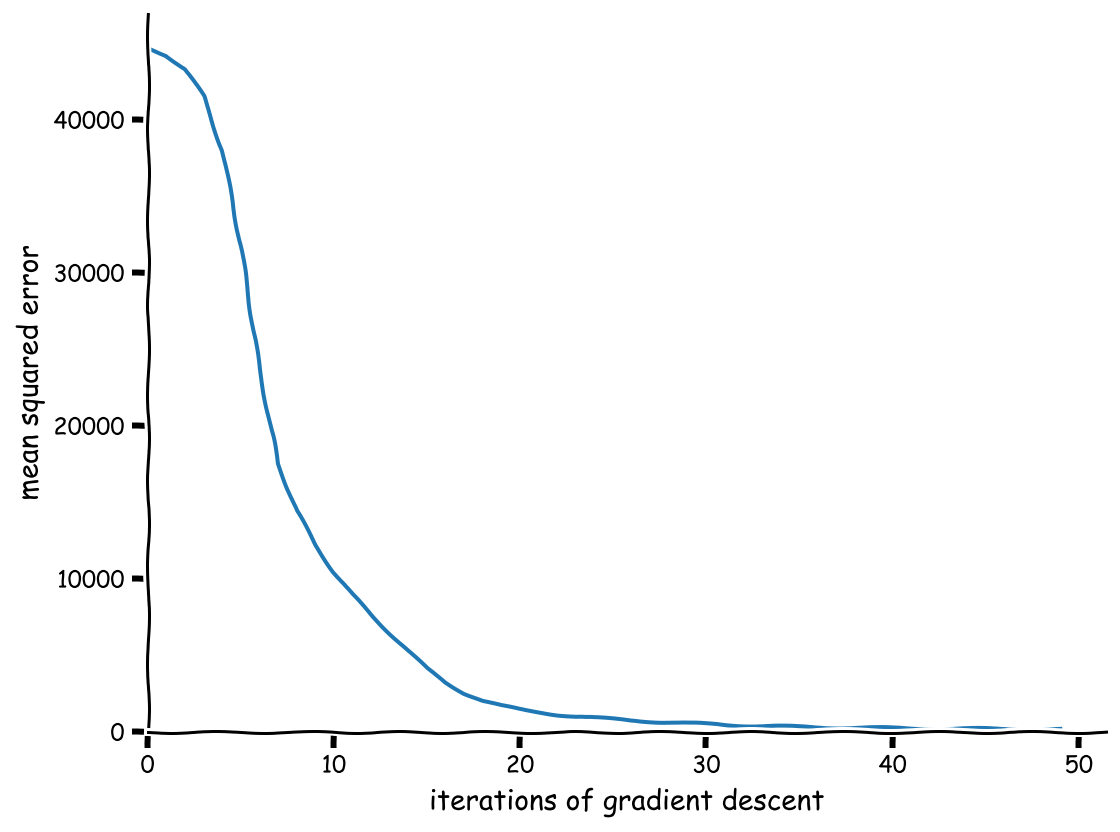
\includegraphics[scale=0.1]{Figures/DL/DLFigure2.png}
\end{subbox}

\end{textbox}
%%%%%%%%%%%%%%%%%%%%%%%%%%%%%%%%%%%%%%%%%%%%%%%%%%%%%%%
%%%%%%%%%%%%%%%%%%%%%%%%%%%%%%%%%%%%%%%%%%%%%%%%%%%%%%%
%%%%%%%%%%%%%%%%%%%%%%%%%%%%%%%%%%%%%%%%%%%%%%%%%%%%%%%
%%%%%%%%%%%%%%%%%%%%%%%%%%%%%%%%%%%%%%%%%%%%%%%%%%%%%%%
\begin{textbox}{\href{https://compneuro.neuromatch.io/tutorials/W2D1_DeepLearning/student/W2D1_Tutorial2.html}{Convolution Neural Network (W2D1T2)} }
\begin{subbox}{subbox}{Introduction to 2D convolutions}
\scriptsize
A 2D convolution is an integral of the product of a filter $f$ and an input image $I$ computed at various positions as the filter is slid across the input. The output of the convolution operation at position $(x,y)$ can be written as follows, where the filter $f$ is size $(K,K)$:
\begin{equation}
C(x,y) = \sum_{k_x=-K/2}^{K/2} \sum_{k_y=-K/2}^{K/2} f(k_x,k_y) I(x+k_x,y+k_y)
\end{equation}
This convolutional filter is often called a kernel.
\end{subbox}
%%%%%%%%%%%%%%%%%%%%%%%%%%%%%%%
\begin{subbox}{subbox}{Convolutional Layers}
\scriptsize
In a fully connected layer, each unit computes a weighted sum over all the input units. In a convolutional layer, on the other hand, each unit computes a weighted sum over only a small patch of the input, referred to as the unit's \textit{receptive field}. When the input is an image, the receptive field can be thought of as a local patch of pixels.
  
In a fully connected layer, each unit uses its own independent set of weights to compute the weighted sum. In a convolutional layer, all the units (within the same channel) share the same weights. This set of shared weights is called the convolutional filter or kernel. The result of this computation is a convolution, where each unit has computed the same weighted sum over a different part of the input. This reduces the number of parameters in the network substantially.

\centering
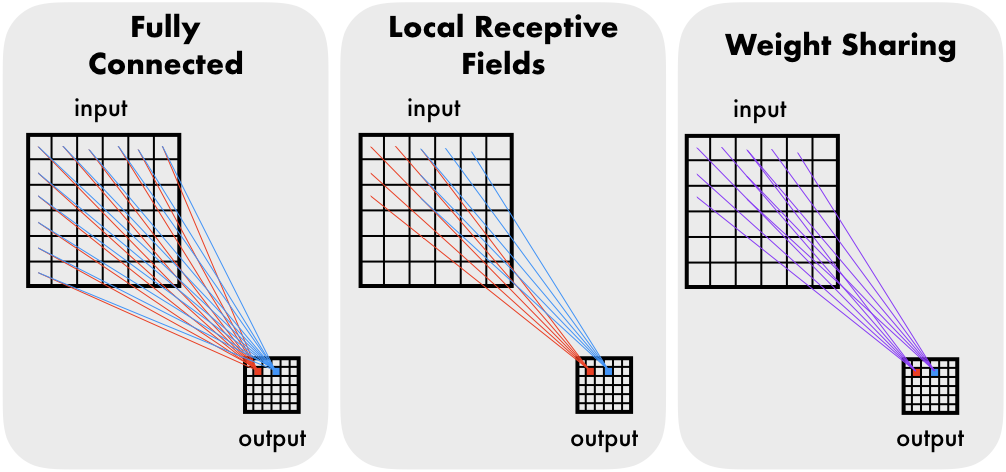
\includegraphics[scale=0.2]{Figures/DL/DLFigure3.png}
\end{subbox}
\end{textbox}
%%%%%%%%%%%%%%%%%%%%%%%%%%%%%%%%%%%%%%%%%%%%%%%%%%%%%%%
%%%%%%%%%%%%%%%%%%%%%%%%%%%%%%%%%%%%%%%%%%%%%%%%%%%%%%%
\begin{textbox}{\href{https://compneuro.neuromatch.io/tutorials/W2D1_DeepLearning/student/W2D1_Tutorial3.html}{Building and Evaluating Normative Encoding Models (W2D1T3)} }
\begin{subbox}{subbox}{Setting up Deep Network and Neural Data}
\scriptsize
We will build our normative encoding model by optimizing its parameters to solve an orientation discrimination task. 

To do this, we will use a convolutional neural network (CNN). Here, we will use a CNN that performs two-dimensional convolutions on the raw stimulus image (which is a 2D matrix of pixels), rather than one-dimensional convolutions on a categorical 1D vector representation of the stimulus. CNNs are commonly used for image processing. 

The particular CNN we will use here has two layers:
\begin{enumerate}
    \item 
a convolutional layer, which convolves the images with a set of filters
    \item a fully connected layer, which transforms the output of this convolution into a 10-dimensional representation
\end{enumerate}

Finally, a set of output weights transforms this 10-dimensional representation into a single scalar $p$, denoting the predicted probability of the input stimulus being tilted right. 

\centering
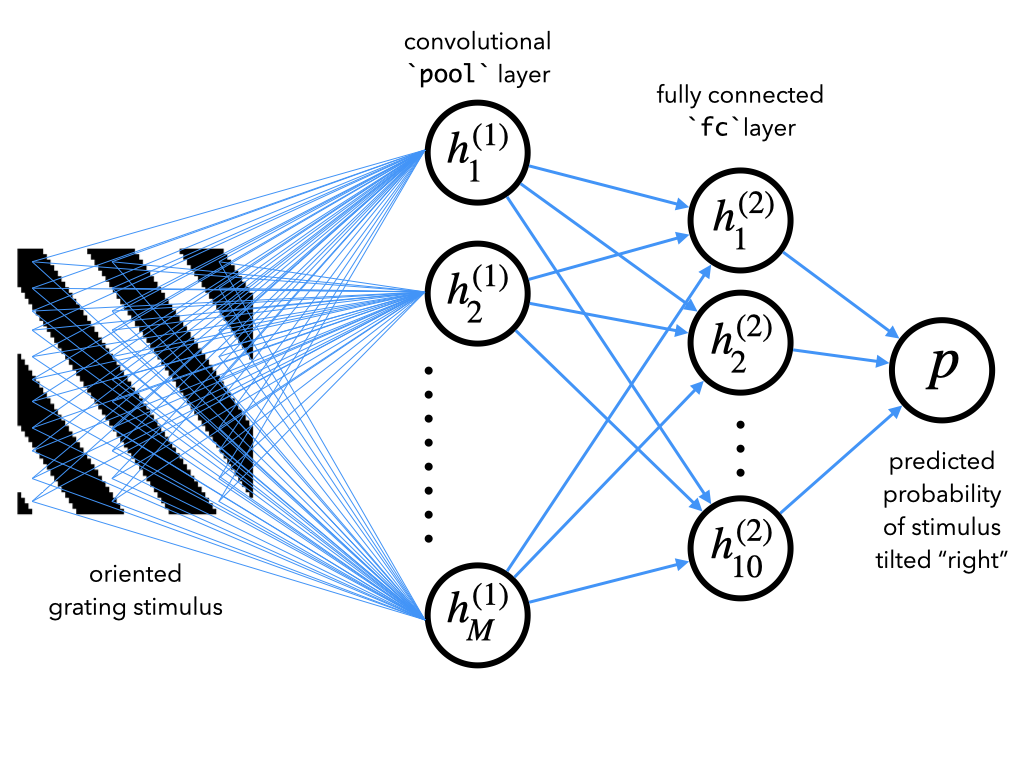
\includegraphics[scale=0.18]{Figures/DL/DLFigure4.png}

\end{subbox}
\end{textbox}
%%%%%%%%%%%%%%%%%%%%%%%%%%%%%%%%%%%%%%%%%%%%%%%%%%%%%%%
%%%%%%%%%%%%%%%%%%%%%%%%%%%%%%%%%%%%%%%%%%%%%%%%%%%%%%%
\begin{textbox}{\href{https://compneuro.neuromatch.io/tutorials/W2D1_DeepLearning/student/W2D1_Tutorial3.html}{Building and Evaluating Normative Encoding Models (W2D1T3)} }
%%%%%%%%%%%%%%%%%%%%%%%%%%%%%%%
\begin{subbox}{subbox}{Representational Dissimilarity matrix (RDM)}
\scriptsize
To quantify this, we begin by computing the representational dissimilarity matrix (RDM) for the mouse V1 data and each model layer. This matrix, which we'll call $\mathbf{M}$, is computed as one minus the correlation coefficients between population responses to each stimulus. We can efficiently compute this by using the $z$-scored responses. 

The $z$-scored response of all neurons $\mathbf{r}$ to stimulus $s$ is the response mean-subtracted across neurons $i$ and normalized to standard deviation 1 across neurons $i$ where $N$ is the total number of neurons:
\begin{equation}
  \mathbf{z}^{(s)} = \frac{\mathbf{r}^{(s)} - \mu^{(s)}}
  {\sigma^{(s)}}
\end{equation}
where $\mu^{(s)} = \frac{1}{N}\sum_{i=1}^N r_i^{(s)}$ and 
$\sigma^{(s)} = \sqrt{\frac{1}{N}\sum_{i=1}^N \left( r_i^{(s)} - \mu^{(s)} \right)^2}$.

Then the full matrix can be computed as:
\begin{gather}
  \mathbf{M} = 1 - \frac{1}{N} \mathbf{ZZ}^T
\end{gather}
where $\mathbf{Z}$ is the z-scored response matrix with rows $\mathbf{r}^{(s)}$ and N is the number of neurons (or units).
\end{subbox}
%%%%%%%%%%%%%%%%%%%%%%%%%%%%%%%
\begin{subbox}{subbox}{Determining Representation Similarity}
\scriptsize
To quantify how similar the representations are, we can simply correlate their dissimilarity matrices. For this, we'll again use the correlation coefficient. Note that dissimilarity matrices are symmetric ($M_{ss'} = M_{s's}$), so we should only use the off-diagonal terms on one side of the diagonal when computing this correlation to avoid overcounting. Moreover, we should leave out the diagonal terms, which are always equal to 0, so will always be perfectly correlated across any pair of RDM's.

\centering
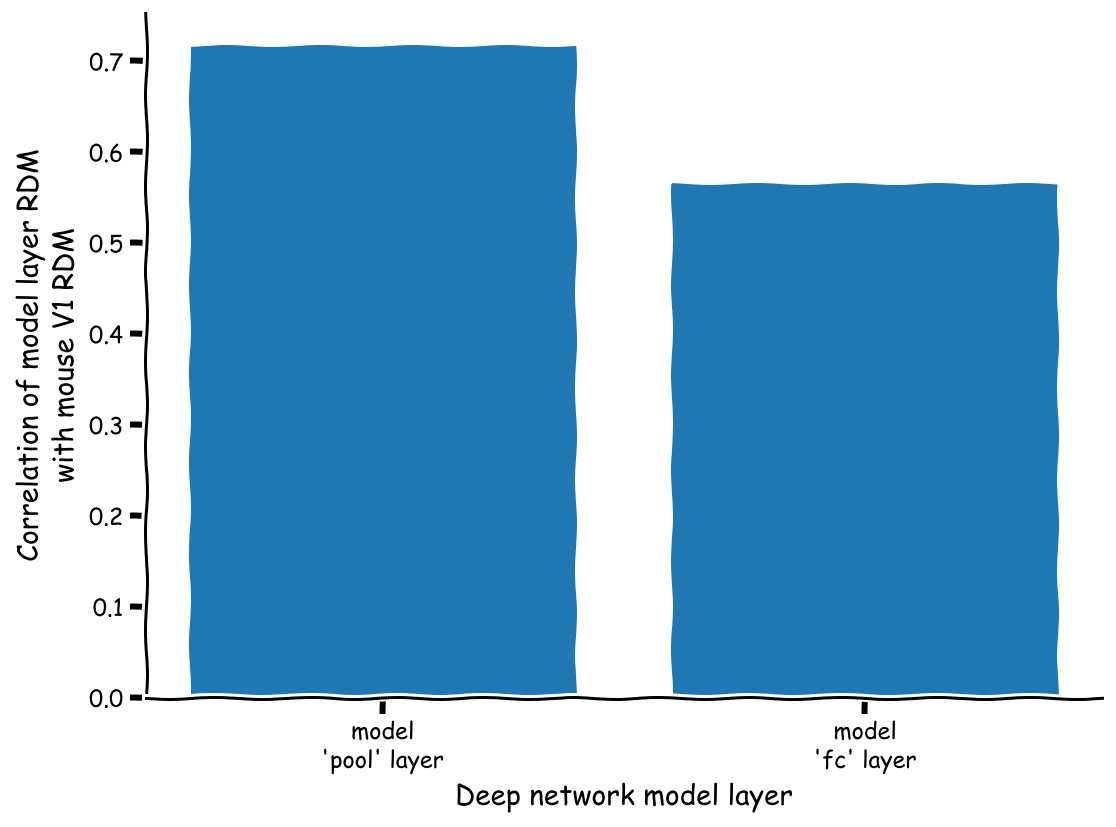
\includegraphics[scale=0.12]{Figures/DL/DLFigure5.png}

\end{subbox}
\end{textbox}

%%%%%%%%%%%%%%%%%%%%%%%%%%%%%%%%%%%%%%%%%%%%%%%%%%%%%%%
%%%%%%%%%%%%%%%%%%%%%%%%%%%%%%%%%%%%%%%%%%%%%%%%%%%%%%%
\begin{textbox}{\href{https://compneuro.neuromatch.io/tutorials/W2D1_DeepLearning/student/W2D1_Tutorial3.html}{Building and Evaluating Normative Encoding Models (W2D1T3)} }
%%%%%%%%%%%%%%%%%%%%%%%%%%%%%%%
\begin{subbox}{subbox}{Qualitative Comparisons of CNNs and Neural Activity}
\scriptsize
To visualize the representations in the data and in each of these model layers, we'll use two classic techniques from systems neuroscience:
\begin{enumerate}
    \item 
 \textbf{tuning curves}: plotting the response of single neurons (or units, in the case of the deep network) as a function of the stimulus orientation

    \item  \textbf{dimensionality reduction}: plotting full population responses to each stimulus in two dimensions via dimensionality reduction. We'll use the non-linear dimensionality reduction technique t-SNE for this. We use dimensionality reduction because there are many units and it's difficult to visualize all of them at once. We use a non-linear dimensionality reduction technique because it can capture complex relationships between stimuli.
\end{enumerate}

\end{subbox}
%%%%%%%%%%%%%%%%%%%%%%%%%%%%%%%
\begin{subbox}{subbox}{Tuning Curves}
\scriptsize
Below, we show some example tuning curves for different neurons and units in the trained CNN.

\centering
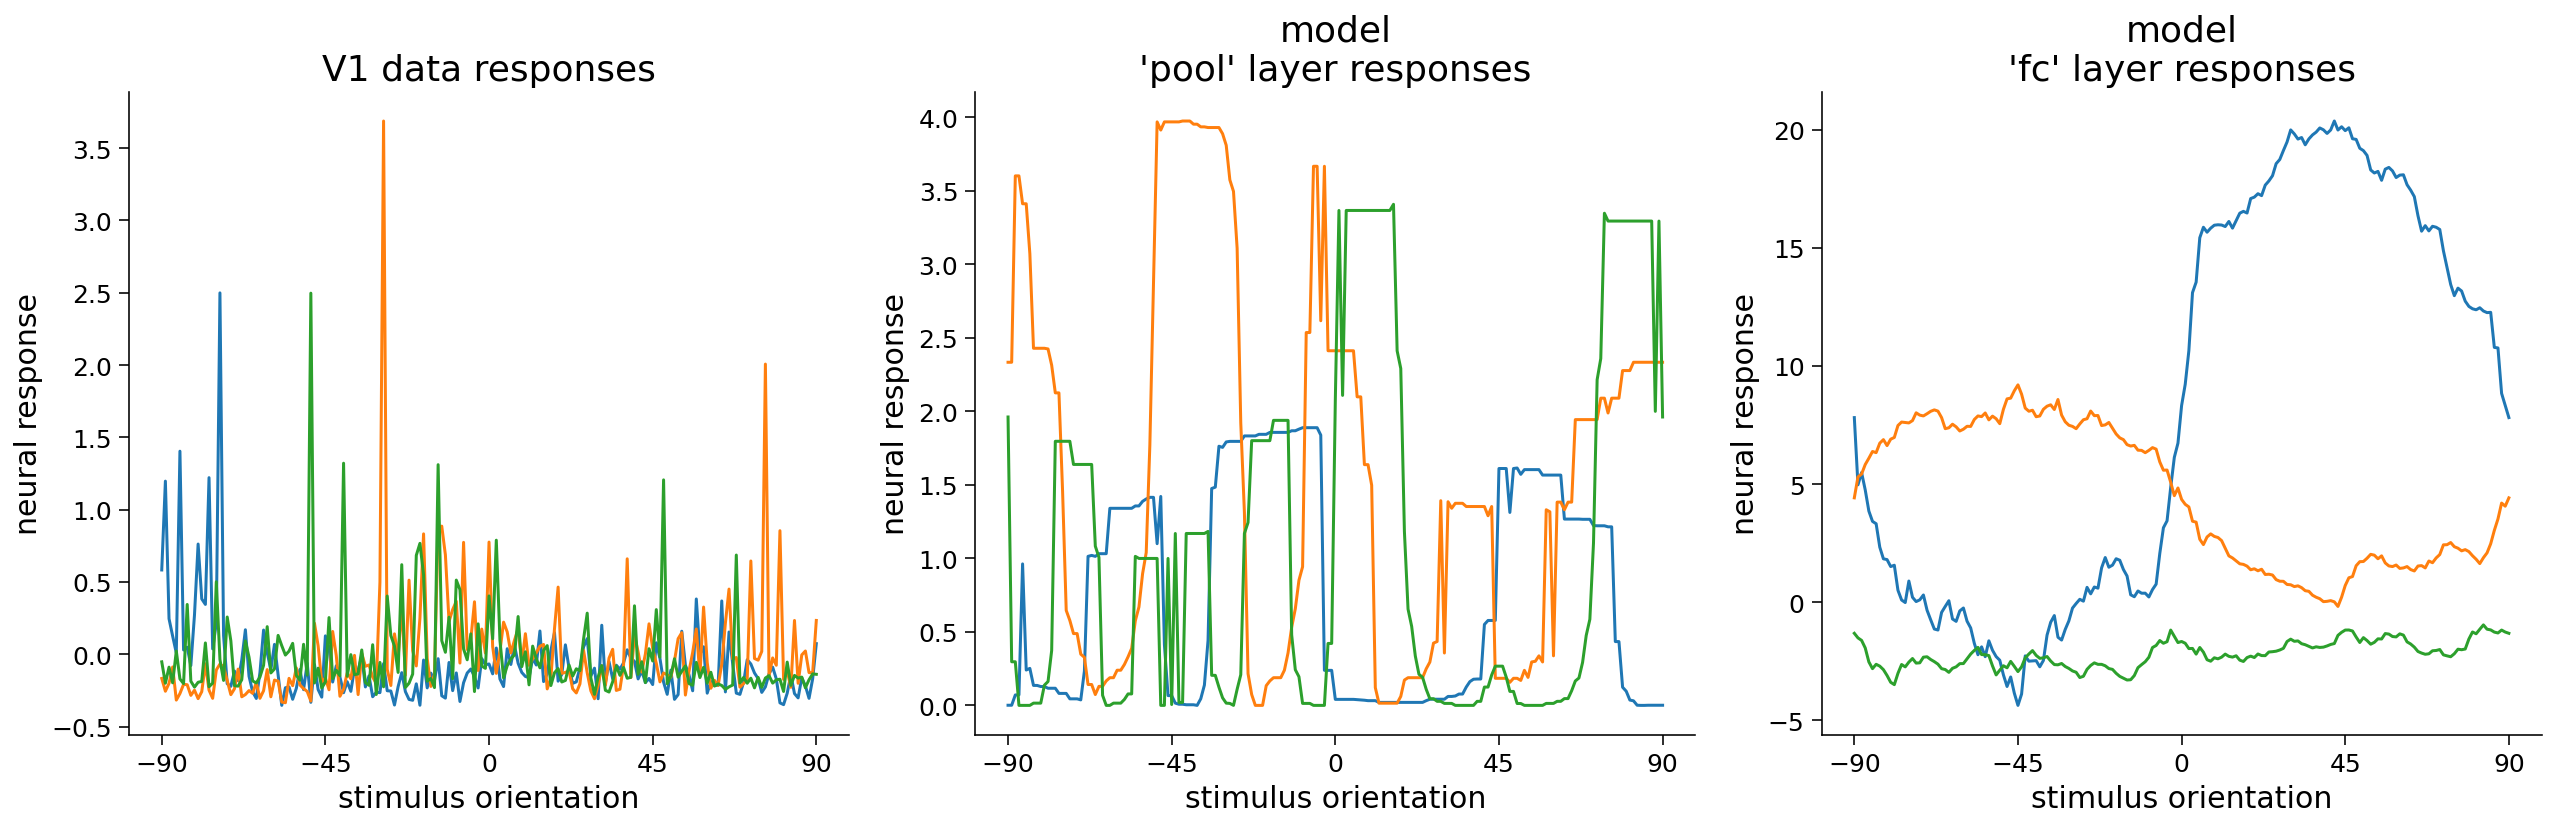
\includegraphics[scale=0.15]{Figures/DL/DLFigure6.png}

\end{subbox}
%%%%%%%%%%%%%%%%%%%%%%%%%%%%%%%
\begin{subbox}{subbox}{Dimensionality Reduction of Representations}
\scriptsize
We can visualize a dimensionality-reduced version of the internal representations of the mouse primary visual cortex or CNN internal representations in order to potentially uncover informative structure. Here, we use PCA to reduce the dimensionality to 20 dimensions, and then use tSNE to further reduce dimensionality to 2 dimensions.

\centering
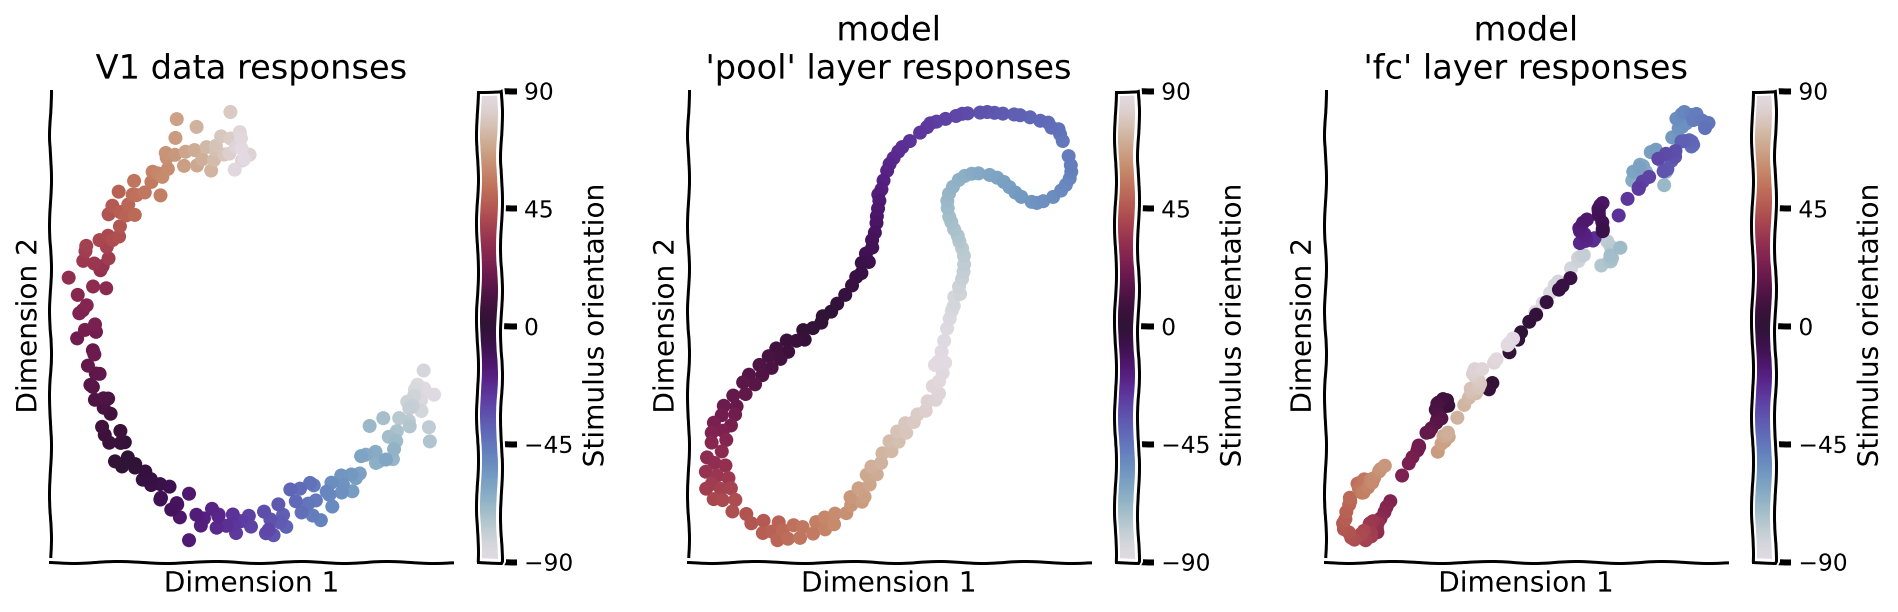
\includegraphics[scale=0.18]{Figures/DL/DLFigure7.png}

\end{subbox}
\end{textbox}
\end{multicols}

\end{document}
